\documentclass[11pt,a4paper,onecolumn,openright,oneside]{report}
\usepackage[square,sort&compress,comma,numbers]{natbib}
\usepackage[sectionbib]{chapterbib}
\usepackage[utf8]{inputenc}
\usepackage[T1]{fontenc}
\usepackage[top=2cm, bottom=2cm]{geometry}
\usepackage{float}%positionner les images
\usepackage{graphicx}%pour les images
\usepackage{soul}
\usepackage{enumitem}
\usepackage{makecell}
\usepackage{url}
\usepackage{tablefootnote}
\usepackage[colorlinks = true,
linkcolor = blue,
urlcolor  = blue,
citecolor = blue,
anchorcolor = blue
hyperfootnotes=false]{hyperref}

 \newcommand{\HRule}{\rule{\linewidth}{0.5mm}} %------- Faire les trai Dans La Page De Garde

%---- Begin Tableau Considérations pour les systèmes relationnels vs NoSQL
\usepackage{array,multirow,makecell} 
\newcolumntype{C}[1]{>{\centering\arraybackslash }b{#1}}
\newcolumntype{F}[1]{>{ \centering \vspace{1.mm} \arraybackslash}m{#1}<{ \vspace{1.mm}\arraybackslash }}
\newcolumntype{R}[1]{>{  \vspace{1.mm} \arraybackslash}m{#1}<{ \vspace{1.mm}\arraybackslash }}
\newcolumntype{G}[1]{>{ \centering \vspace{2.mm} \arraybackslash}m{#1}<{ \vspace{2.mm}\arraybackslash }}
%---- End Tableau Considérations pour les systèmes relationnels vs NoSQL

%------- Begin Ajouter les subsubsection à la table des matiere--------
\addtocounter{tocdepth}{3}
\setcounter{secnumdepth}{3}
%------- end Ajouter les subsubsection à la table des matiere--------

\usepackage{footnote} %------ Pur ressortir les note des élèment du tableau

\usepackage[french]{babel}

\usepackage{fancyhdr}

\usepackage{adjustbox}% pour orionté le tab 90°
\usepackage{amssymb}% pour chekmark dans le tableau
\makesavenoteenv{tabular}


\begin{document}
	\setcellgapes{3pt}
	
	\begin{titlepage}
		
		\begin{center}
			
			\textsc{\LARGE République Algérienne Démocratique et Populaire}\\
			\textsc{\LARGE Ministère de l’Enseignement Supérieur et de la Recherche Scientifique}\\
			\textsc{\LARGE Université Mouloud Mammeri de Tizi-Ouzou}\\
			
			\begin{figure}[H]
				\centering
				
\includegraphics[scale=1.5]{ummto.PNG}
			\end{figure}
			
			\textsc{\Large En vue de l’obtention du diplôme de Master Academique}\\
			\textsc{\Large Spécialité : Informatique}\\
			\textsc{\Large Options : Systèmes Informatiques et Ingénierie Des Systèmes d’information}\\[1cm]
			
			
			\textsc{\Large Thème}\\
			\HRule \\[0.5cm]
			% { \huge \bfseries Mise en place d'une solution web ERP \\
			% 	Cas: Œuvres Universitaires \\[0.4cm] }
            { \huge \bfseries Implémentation d'une solution web ERP \\
				Cas: Œuvres Universitaires \\[0.4cm] }
			
			\HRule \\[0.5cm]
			
			
			\emph{Présenté par :}\\
			
			Yanis \textsc{OUERDANE}\\
			Mohand \textsc{OURAD}\\[1.5cm]
			
			\emph{Devant le jury composé de :}\\
			
			\leftskip=4.5cm
			Président(e) : M$^{me}$ / M$^{elle}$ / M$^{r}$ JOHN Doe \\
			Examinateur(trice) : M$^{me}$ / M$^{elle}$ / M$^{r}$ DOE John\\
			Promoteur(trice) : M$^{me}$ \textsc{Goumeziane} Lynda \\ [1.5cm]
			
			
			\vfill
            {\large Année universitaire: 2020/2021}
			
		\end{center}
		
	\end{titlepage}

	\chapter*{\huge Remerciements}
	
	\begin{center}
		\it \Large
		D’abord, nous remercions le bon \textbf{DIEU} de nous avoir donné santé et courage pour réaliser ce travail.\\
		
		Nous tenons à exprimer notre profonde gratitude à notre encadreur \textbf{Mme GOUMEZIANE Lynda}, pour nous avoir encadré et guidé et surtout pour ses judicieux conseils qui ont contribué à alimenter notre réflexion.\\
		
		Nous remercions chaleureusement les membres de jury pour l’honneur qu’ils nous ont fait en acceptant de juger notre travail.\\
		
		Nos sincères sentiments vont à nos parents qui ont sacrifié jusqu’aujourd’hui et leurs encouragements tout le long de notre parcours.\\
		
		\leftskip=10cm 
		
		Yanis, Mohand.
		
		\leftskip=0cm
		
	\end{center}
	%------------------- End Remerciement ----------------------------
	
	\chapter*{\huge Dédicaces}
	
	\begin{center}
		\it \Large
		Je dédie ce modeste travail :
		A mes très chers parents que dieu les
		protègent, pour leur aide et leur soutien tout au long
		de mes études,\\
		
		A toute ma famille, à mes chers amis,\\
		
		Enfin à tous ceux qui ont contribué de près
		ou de loin pour la réalisation de ce travail.\\
		
		\leftskip=12cm
		
		Yanis.
		
		\leftskip=0cm
		
	\end{center}
    \chapter*{\huge Dédicaces}
	
	\begin{center}
		\it \Large
		Je dédie ce modeste travail :
		A mes très chers parents que dieu les
		protègent, pour leur aide et leur soutien tout au long
		de mes études,\\
		
		A toute ma famille, à mes chers amis,\\
		
		Enfin à tous ceux qui ont contribué de près
		ou de loin pour la réalisation de ce travail.\\
		
		\leftskip=12cm
		
		Mohand.
		
		\leftskip=0cm
		
	\end{center}
	
	\tableofcontents
	\listoffigures
	\listoftables

	\pagestyle{fancy}
	\fancyhead{}
	
	\renewcommand{\chaptermark}[1]{\markboth{\bsc{\chaptername~\thechapter{} :} #1}{}}
	
	\rhead[\textsl{\leftmark}]{\textsl{\rightmark}}
	\lhead[\textsl{\rightmark}]{\textsl{\leftmark}}
	
	\renewcommand{\headrulewidth}{1.2pt}
	
	\newcommand\blfootnote[1]{
		\begingroup
		\renewcommand\thefootnote{}\footnote{#1}
		\addtocounter{footnote}{-1}
		\endgroup
	}
        \part{Solutions Web}
            \chapter{Les Œuvres Universitaires}

\section{Introduction}
    Notre projet comprend la conception et la réalisation d'une application d'aide à la gestion des transports, de la restauration, des dossiers de bourse et des dossiers de d'hébergement. A cet effet, il est nécessaire de présenter la direction des oeuvres universitaires (D.O.U) de Tizi Ouzou en tant qu'organisme d'accueil et chaque service fourni par cette dernière afin de comprendre leurs principales activités.\\

\section{Présentation de la D.O.U}
    Placée sous la tutelle de l’office national des œuvres universitaires et du ministère de l’enseignement supérieur et de la recherche scientifique. Elle est créée en vertu de l’arrêté interministériel du 22/12/2004 portant la création des directions des œuvres universitaires. La direction est chargée de la gestion des Résidences Universitaires de la wilaya en assurant au profit des étudiants différentes prestations de services en matière d’hébergement, transport, restauration, activités scientifiques, culturelles et sportives, prévention sanitaire, et bourse.\\

\section{Missions et activités de la D.O.U}
    Sa principale mission est de promouvoir la politique de l'état visant à améliorer la vie quotidienne de l'étudiant universitaire à travers un ensemble de services tels le soutien financier, l'hébergement, le transport, la restauration, et tout cela dans un cadre agréable à l'intérieur des Résidences Universitaires grâce à un riche programme d'activités culturelles, scientifiques et sportives, sans oublier bien sûr une protection sanitaire assurée par une équipe médicale et paramédicale professionnelle. Elle assure plus précisément les activités suivantes :\\
    \begin{itemize}
        \item La prise en charge totale en matière d’application de la politique nationale des œuvres universitaires.
        \item Le contrôle et la coordination entre les résidences universitaires.
        \item De veiller à l’amélioration des conditions de vie de l’étudiant à l’intérieur de la résidence universitaire.
        \item La gestion des bourses.
        \item L’élaboration du plan de transport des résidences universitaires et le suivi de son exécution.
        \item La promotion des activités scientifiques, culturelles, sportives et loisirs.
        \item Assurer hygiène et sécurité.
        \item L’accueil et l’orientation des nouveaux bacheliers.
    \end{itemize}

\section{Organigramme de la D.O.U}
    L’organigramme de la direction des œuvres universitaires est présenté dans le tableau suivant :
    %_____________________________________ figure 1____________
    \begin{figure}[H]
        \centering
            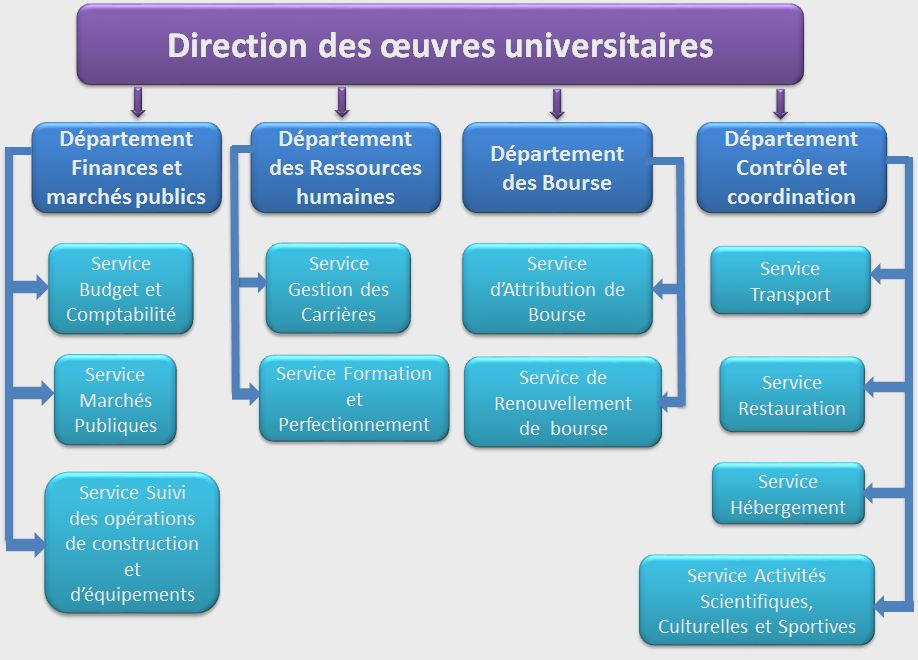
\includegraphics[scale=0.4]{chapitre1/direction-diag.jpg}
        \caption{Organigramme de la D.O.U}
    \end{figure} 
    %__________________________________________________________

\section{L’organisation de la D.O.U}
    La direction des œuvres universitaires de béjaia est composée de 04 départements selon le schéma suivant :

\subsection{Le département des ressources humaines}
    \begin{itemize}
        \item Service de la gestion des carrières
        \item Service de la formation et de perfectionnement\\
    \end{itemize}

    Il est chargé de :
    \begin{itemize}
        \item Gérer la carrière des personnels relevant de la direction des œuvres universitaires
        \item Assurer la mise en œuvre des plans de formation et du perfectionnement des personnels relevant de la direction des œuvres universitaires
    \end{itemize}

\subsection{Le département du controle et de la coordination}
    \begin{itemize}
        \item Service du transport
        \item Service de la restauration
        \item Service hébergement
        \item Service des activité scientifiques, culturelles et sportives\\
    \end{itemize}

    Il est chargé de :
    \begin{itemize}
        \item Elaborer les plans de transport universitaire concernant les résidences universitaires rattachées a la DOU et de suivre leur mise en œuvres
        \item Suivre, contrôler et coordonner les activités d'œuvre universitaires     assurées par les résidences universitaires rattachées a la DOU
        \item Proposer toute mesure de rationalisation de l'utilisation des moyens   humains, matériels et financiers   consacrés   aux  activités   des   œuvres universitaires
        \item Examiner les programmes d'activités scientifiques, et sportives et veiller  au suivi de leur application après leur approbation par le directeur de la direction
    \end{itemize}

\subsection{Le département des bourses}
    \begin{itemize}
        \item Service de l'attribution des bourses
        \item Service du renouvellement des bourses\\
    \end{itemize}

    Il est chargé de :
    \begin{itemize}
        \item Assurer le traitement et le suivi des dossiers des étudiants bénéficiaires de bourses
        \item Assurer le paiement régulier des bourses
        \item Assurer le traitement et la prise en charge des bourses des étudiants étrangers
    \end{itemize}

\subsection{Le département des finances et des marchés publics}
    \begin{itemize}
        \item Service du budget et de la comptabilité
        \item Service des marchés publics
        \item Service du suivi des opérations de construction et de l'équipement\\
    \end{itemize}

    Il est chargé de :
    \begin{itemize}
        \item Gérer les moyens matériels et financiers mis a la disposition de la direction des oeuvres universitaires
        \item Assurer le service de traitements des personnels de la direction
        \item Assurer la prise en charge des différents étapes de passation des marchés publics et d'en suivre l'exécution par les résidences universitares
        \item Assurer en liaison avec les services concernés le suivi des  opérations de construction et d'équipement des résidences universitaires
    \end{itemize}

\section{Historique et  statistiques}
\leftskip=1cm

L'expression " Big Data " apparaît fréquemment dans la presse et dans les revues universitaires, et des programmes de "Data Science» ont vu le jour dans le monde universitaire au cours des six dernières années. Le 29 mars 2012, WHOSTP\footnote{White House Office of Science and Technology Policy en français Le Bureau de la politique scientifique et technologique de la Maison Blanche} a annoncé la "Big Data Research and Development Initiative" qui s'appuie sur des initiatives fédérales "allant de l'architecture informatique et des technologies de mise en réseau aux algorithmes, à la gestion des données, à l'intelligence artificielle, apprentissage automatique, développement et déploiement de cyber infrastructures avancées"  \cite{ridgeway2018policing}.\\

Les "Big data" sont apparues environ 560 fois par an dans JSTOR\footnote{JSTOR est à la fois un système d'archivage en ligne de publications universitaires et scientifiques }\blfootnote{et une bibliothèque numérique payante. Fondé en 1995, JSTOR est aujourd'hui une société }\blfootnote{américaine à but non lucratif basée à New York} de 2014 à 2017, même si elles ont été mentionnées moins d'une fois par an au siècle avant 2000 et seulement en moyenne environ huit fois par an entre 2001 et 2010.\\

Au cours des six dernières années, au moins 17 programmes de science des données ont commencé dans les principales universités de recherche américaines et Internet regorge de publicités pour des livres et des cours de science des données.\\

Selon l’étude Data Age 2025\footnote{L'étude Data Age 2025 est une étude sur la digitalisation dans le monde réalisée par l'IDC, établi}\blfootnote{ un comparatif de la digitalisation dans quatre régions (Asie/Pacifique, dont Japon, mais hors Chine) ; }\blfootnote{Chine ; États-Unis ; EMEA (Europe, Moyen-Orient et Afrique).} La sphère de données mondiale passera de 33 zettaoctets en 2018 à 175 Zo d'ici 2025. Près de 30\% des données mondiales devront être traitées en temps réel et le stockage réalisé sur le Cloud public représentera 49\% du volume total de données \cite{dataage2025}.\\

La figure suivante permet de représenter la quantité de données générée en 60 secondes d’Internet en 2020:\\

%_____________________________________ figure 1____________
\begin{figure}[H]
 \centering
 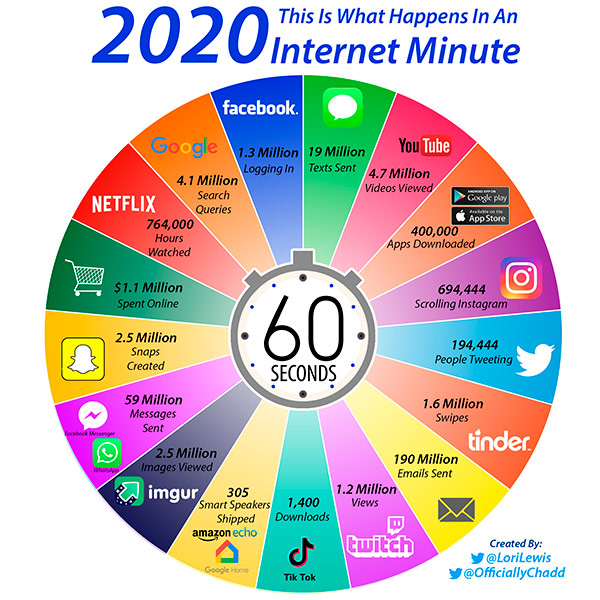
\includegraphics[scale=0.5]{chapitre1/1-MinuteInternet2020.PNG}
 \caption{1 minute d'internet en 2020}
\end{figure} 
%__________________________________________________________


En analysant la figure 1.1 on constate l’énorme quantité de données qui circule. En effet, cette année à chaque minute d’Internet, sont envoyés plus de 59 millions de messages. Chaque minute, Google enregistre près de 4,1 millions de requêtes différentes sur son moteur de recherche. Facebook enregistre près de 1,3 de logins.\\ 

\leftskip=0,5cm


%Subsection----------------- Quelques définitions liées au Big Data ---------
\section{Quelques définitions liées au Big Data}
\leftskip=0,5cm

% Aucune définition précise ou universelle ne peut être donnée au Big Data. Etant un objet complexe polymorphe, sa définition varie selon les communautés qui s’y intéressent en tant qu’usager ou fournisseur de services.\\
 
% \textbf{Définition 1.} Le Big Data désigne l'ensemble des données numériques produites par l'utilisation des nouvelles technologies à des fins personnelles ou professionnelles. Cela regroupe les données d'entreprise? des contenus publiés sur le web, des transactions de commerce électronique, des échanges sur les réseaux sociaux, des données transmises par les objets connectés des données géolocalisées, ...etc \cite{futura-sciences}. \\

% \textbf{Définition 2.} Le "Big Data" désigne les technologies et les initiatives qui impliquent des données trop diverses, en évolution rapide ou massives pour que les technologies, les compétences et les infrastructures conventionnelles puissent être traitées efficacement. Autrement dit, le volume, la vitesse ou la variété des données est trop important \cite{bigdatamongo}. \\

% \textbf{Définition 3.} Le terme Big Data fait référence aux données dont le coût de stockage, de gestion et d'analyse dans des systèmes de base de données traditionnels (relationnels et/ou monolithiques) serait généralement trop élevé. Habituellement, ces systèmes ne sont pas rentables, car ils ne disposent pas de la flexibilité nécessaire pour stocker des données non structurées (comme des images, du texte et des vidéos), pour accommoder des données "à haute vélocité" (en temps réel) ou pour s'adapter automatiquement à de très gros volumes de données (de l'ordre du pétaoctet) \cite{Google-Cloud}.\\





% %Subsection----------------- Intérêts du Big Data ---------
% \section{Intérêt du Big Data}
% \leftskip=0,5cm

% L’information est l’arme fatale du XXIème siècle. Celui qui détient l’information, a le pouvoir. C’est ce que nous répètent tous les experts géopolitiques et tous les économistes. Le Big Data en est maintenant la plus grande source et il est désormais généré tout autour de nous.\\

% Avec la croissance de l’Internet des objets, l’utilisation des smartphones, des médias sociaux des applications dans le cloud et autres technologies d’intelligence artificielle, le Big Data est devenu plus important que jamais et cela au sein de plusieurs secteurs d’activité mais plus principalement au niveau des services marketing. Plusieurs entreprises et organisations de toutes tailles utilisent maintenant le Big Data comme moyen d’obtenir davantage d’informations pour :\\

% \leftskip=1cm
% \begin{itemize}\renewcommand{\labelitemi}{$\bullet$}
% 	\item Améliorer les offres de l'entreprise en offrant une analyse complète du comportement et des attentes du consommateur.\newpage
% 			\emph{\textbf{Exemple:}} \emph{Google Analytics\footnote{Google Analytics est un service gratuit d'analyse d'audience d'un site Web ou d'applications utilisé}\blfootnote{ par plus de 10 millions de sites, soit plus de 80 \% du marché mondial} permet par exemple d’optimiser un site web par une analyse en temps réel des données liées: nombre de visites, comportement de navigation, taux de rebond, nombre de pages lues, taux de clics..etc
% }\\ 
  
%   \item Anticiper les besoins et la demande des clients et adapter ainsi les campagnes marketing.
% 	  \\ \\
% 			\emph{\textbf{Exemple:}} \emph{La consultation d'appareils photos sur le site de la Fnac\footnote{La Fnac « Fédération nationale d'achats », puis « Fédération nationale d'achats des cadres ») }\blfootnote{est une chaîne de magasins française spécialisée dans la distribution de produits culturels et }\blfootnote{électroniques à destination du grand public} et le fait de retrouver des bannières d’appareils photo sur tous les sites que l'on fréquente est un avantage du Big Data (certains diront que c’est plutôt un inconvénient… !).}\\ 
	
%   \item Prédire des faits ou générer des statistiques futur.
% 	 \\ \\
% 			\emph{\textbf{Exemple:}} \emph{Target\footnote{Target Corporation, située à Minneapolis dans le Minnesota est une entreprise de grande}\blfootnote{ distribution. Elle est le deuxième plus gros distributeur discount et le cinquième distributeur général }\blfootnote{aux États-Unis}, aux Etats-Unis, parvient avec le Big Data à prédire l’accouchement prochain de femmes enceintes.}\\ 
	
%   \item Optimiser la logistique et l'organisation.
% 	 \\ \\
% 			\emph{\textbf{Exemple:}} \emph{Il permet, par exemple, de suivre les ventes en temps réel et donc d’optimiser la gestion des stocks. Amazon\footnote{Amazon est une entreprise de commerce électronique américaine basée à Seattle. Elle est un des }\blfootnote{géants du Web, regroupés sous l'acronyme GAFAM5, aux côtés de Google, Apple, Facebook et }\blfootnote{Microsoft.} teste même régulièrement des fonctionnalités de livraison intuitive, visant à proposer la livraison à la commande.
% .}\\ 
	
% \item Le Big Data permet aussi de réduire les coût d'organisation et d'augmenter la productivité, de fidéliser la marque en analysant les comportement de prospects et des clients et améliore l'expérience de ces derniers.\\
% \end{itemize}


% \leftskip=0,5cm
% pour résumer, Le Big Data permet de construire de meilleurs modèles, qui produisent des résultats plus précis avec  des approches extrêmement innovantes concernant la manière dont :\\

%   \leftskip=1cm
% 	\begin{itemize}\renewcommand{\labelitemi}{$\bullet$}
% 		\leftskip=1cm \item Les entreprises se commercialisent et vendent leurs produits.
% 		\leftskip=1cm \item La gestion des ressources humaines. 
% 		\leftskip=1cm \item La réaction au catastrophes naturelles.\\
% 	\end{itemize}
	
% \leftskip=0,5cm
% Ces exemples ne sont finalement qu’une poignée des opportunités qu’offre le Big Data. Les entreprises, et pas seulement, devront faire preuve d’imagination, d’organisation et d’un énorme sens d’analyse pour prendre la pleine mesure du phénomène. De cette maîtrise découle de nouveaux usages qui bouleverse notre façon de concevoir Internet.
% \newpage
% Mais le Big Data, ce n’est pas que des avantages. C'est aussi des contraintes, nous verrons ces dernières dans la section suivante.

% %Subsection----------------- Les contraintes du Big Data---------
% \section{Les contraintes du Big Data}
% \leftskip=0,5cm

% L'idée est de comprendre que les entreprises et les organisations collectent et exploitent de grands volumes de données pour améliorer leurs produits finaux, que ce soit la sécurité, la fiabilité, les soins de santé ou la gouvernance. En général, dans les affaires, l'objectif est de transformer autant de données en une forme d'avantage commercial. La question est de savoir comment utiliser des volumes de données plus importants pour améliorer la qualité de notre produit final? Malgré un certain nombre de défis qui y sont liés.\\

% Certaines publications \cite{labrinidis2012challenges} discutent des obstacles au développement d'applications de mégadonnées. Les principaux défis sont énumérés comme suit :\\

% \begin{itemize}[label=\textbullet]


% \item \textbf{Représentation des données :} De nombreux ensembles de données présentent certains niveaux d'hétérogénéité dans le type, la structure, la sémantique, l'organisation, la granularité et l'accessibilité. La représentation des données vise à rendre les données plus significatives pour l'analyse informatique et l'interprétation des utilisateurs. Néanmoins, une représentation incorrecte des données réduira la valeur des données originales et peut même empêcher une analyse efficace des données.\\
% \item \textbf{Réduction de la redondance et compression des données :} En général, il existe un niveau élevé de redondance dans les jeux de données. La réduction de la redondance et la compression des données sont efficaces pour réduire le coût indirect de l'ensemble du système en partant du principe que les valeurs potentielles des données ne sont pas affectées. Par exemple, la plupart des données générées par les réseaux de capteurs sont hautement redondantes.\\

% \item \textbf{Gestion du cycle de vie des données :} Par rapport aux progrès relativement lents des systèmes de stockage, la détection et le calcul omniprésents génèrent des données à des taux et des échelles sans précédent. Nous sommes confrontés à de nombreux défis urgents, dont l'un est que le système de stockage actuel ne peut pas supporter des données aussi massives. De manière générale, les valeurs cachées dans le Big Data dépendent de la fraîcheur des données. \\

% \item \textbf{Mécanisme analytique :} Le système analytique des mégadonnées traitera des masses de données hétérogènes dans un temps limité. Cependant, les SGBDR traditionnels sont strictement conçus avec un manque d'évolutivité et d'extensibilité, ce qui ne pourrait pas répondre aux exigences de performance. Les bases de données non relationnelles ont montré leurs avantages uniques dans le traitement des données non structurées et ont commencé à se généraliser dans l'analyse des mégadonnées. Même ainsi, il existe encore quelques problèmes de bases de données non relationnelles dans leurs performances et applications particulières. Des recherches supplémentaires sont nécessaires sur la base de données en mémoire et des échantillons de données basés sur une analyse approximative.\\

% \item\textbf{Confidentialité des données :} La plupart des fournisseurs ou propriétaires de services de mégadonnées ne pouvaient actuellement pas maintenir et analyser efficacement des ensembles de données aussi énormes en raison de leur capacité limitée. Ils doivent s'appuyer sur des professionnels ou des outils pour analyser ces données, ce qui augmente les risques potentiels pour la sécurité. Par exemple, l'ensemble de données transactionnelles comprend généralement un ensemble de données d'exploitation complètes pour piloter les processus métier clés. Ces données contiennent des détails et certaines informations sensibles telles que les numéros de carte de crédit. \\

% \item\textbf{Gestion de l’énergie :} La consommation d'énergie des systèmes informatiques a beaucoup attiré l'attention du point de vue économique et environnemental. Avec l'augmentation du volume de données et des demandes analytiques, le traitement, le stockage et la transmission de données massives consommeront inévitablement de plus en plus d'énergie électrique.\\
% \item\textbf{Expendabilité et évolutivité :} Le système analytique du Big Data doit prendre en charge les ensembles de données présents et futurs. L'algorithme analytique doit être capable de traiter des ensembles de données de plus en plus étendus et plus complexes.\\
% \item\textbf{Coopération :} L'analyse du Big Data est une recherche interdisciplinaire, qui nécessite la coopération d'experts dans différents domaines pour exploiter le potentiel du Big Data.
% Une architecture de réseau Big Data complète doit être mise en place pour aider les scientifiques et les ingénieurs dans divers domaines à accéder à différents types de données et à utiliser pleinement leur expertise, afin de coopérer pour atteindre les objectifs analytiques.

% \end{itemize}


% %Subsection----------------- Les caractéristiques du Big Data ---------
% \section{Les caractéristiques du Big Data}
% \leftskip=0,5cm


% Les mégadonnées sont un terme générique utilisé pour désigner toute collection de données volumineuse et complexe qui peuvent dépasser la capacité de traitement des systèmes et techniques de gestion de données conventionnels. Les applications du Big Data sont infinies.\\

% Les mégadonnées sont souvent caractérisées par \textbf{le volume} extrême des données, la grande \textbf{variété} de types de données et \textbf{la vitesse} à laquelle les données doivent être traitées.(Ces caracteristique sont dites les 3V)\\

% Ces caractéristiques ont été identifiées pour la première fois par l'analyste \textbf{Douglas Laney's} membre du Gartner\footnote{Le Gartner est une entreprise américaine de conseil et de recherche dans le domaine des techniques avancées. Elle mène des recherches, fournit des services de consultation, tient à jour différentes statistiques et maintient un service de nouvelles spécialisées.} dans un rapport publié en 2001. Plus récemment, plusieurs autres caractéristiques(autres V) ont été ajoutées aux descriptions des mégadonnées, notamment \textbf{la véracité}, \textbf{la valeur} et \textbf{la variabilité}. Bien que les mégadonnées ne correspondent à aucun volume de données spécifique, le terme est souvent utilisé pour décrire des téraoctets, des pétaoctets et même des exaoctets de données capturées au fil du temps.\\


% %_____________________________________ figure 1.2____________
% \begin{figure}[H]
%  \centering
%  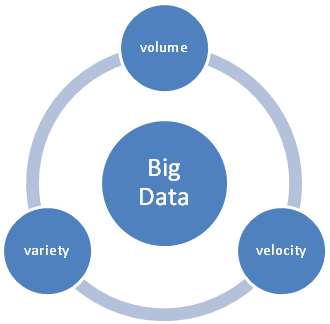
\includegraphics[width=3.5in,scale=1,height=3.5in]{chapitre1/2-3VsOfBigData.PNG}
%  \caption{Les 3V du Big Data}
% \end{figure} 
% %__________________________________________________________

% Certaines personnes attribuent encore plus de V aux Big Data; data scientist et les consultants ont créé diverses listes contenant entre sept et 10 V.\\
% On donne dans ce qui suit 10 caractéristiques "10V" sur les megadonnées sachant que Les 3 premier critères basiques du Big Data sont \textbf{le volume} \textbf{la vitesse} ainsi que \textbf{la variété}:


  
%   \begin{enumerate}
	
	  
%     \item\textbf{Le Volume } Volume :
		
	

% Le volume fait référence aux vastes quantités de données générées chaque seconde, en minutes, en heures et en jours dans notre monde numérisé et qui peuvent provenir de vastes ensembles de données partagés ou de nombreuses petites données et événements collectés au fil du temps. En résumé, le volume est la dimension du Big Data liée à sa taille et à sa croissance exponentielle.\\

% Les défis liés à l'utilisation de volumes de mégadonnées incluent le coût, l'évolutivité et les performances liées à leur stockage, leur accès et leur traitement \cite{seagate2}.\\

% 	  \textit{\textbf{Exemple : }300 heures de vidéo sont mise en ligne sur YouTube chaque minute.} \\
	  
		 
%      \item\textbf{La Variété } Variety :\\


% Elle fait référence aux différentes formes toujours croissantes que les données peuvent prendre, en effet les données Big Data ne sont pas seulement des nombres, des dates et des chaînes. Les mégadonnées englobent également une grande variété de types de données, y compris des données structurées dans des bases de données SQL et des entrepôts de données, des données non structurées, telles que des fichiers texte et document conservés dans des clusters Hadoop ou des systèmes NoSQL, et des données semi-structurées, telles que des journaux de serveur Web ou la diffusion des données à partir de capteurs \cite{bigdatamongo}.\newpage

% \leftskip=0,5cm
% \emph{\textbf{Exemple:}}\emph{ Un projet d'analyse des mégadonnées peut tenter d'évaluer le succès d'un produit et les ventes futures en corrélant les données de ventes passées, les données de retour et les données de révision des acheteurs en ligne pour ce produit.} \\

% 		 \leftskip=0cm
%      \item\textbf{La Vitesse}  Velocity :\\
		

% Elle Fait référence à la vitesse à laquelle les données sont générées et à la vitesse à laquelle les données se déplacent d'un point au suivant.
% Les progrès technologiques ont provoqué une production de données à grande échelle à grande vitesse. Les données en streaming au rythme sans précédent doivent être traitées en temps opportun. Le traitement de ces données en temps réel pour correspondre à leur taux de production est le principal objectif de l'analyse du Big Data.\\
% La vélocité est également importante car l'analyse des mégadonnées s'étend à des domaines tels que l'apprentissage automatique et l'intelligence artificielle (IA), où les processus analytiques trouvent automatiquement des modèles dans les données collectées et les utilisent pour générer des informations.\\

% \leftskip=0,5cm
% \emph{\textbf{Exemple:}}\emph{  Facebook est un exemple très courant d'un environnement qui traite des données à grande vitesse et à grand volume. Selon les enregistrements de janvier 2020, 5 milliards de commentaires sont laissés sur les pages Facebook chaque mois, Le bouton J'aime de Facebook a été enfoncé 1,13 billion de fois.Toutes les 60 secondes, 317 000 mises à jour de statut, 147 000 photos téléchargées, et 54 000 liens partagés \cite{Omnicore} \cite{zephoria}.} \\

% \leftskip=0cm
% \textbf{Remarque: }De plus en plus de \textbf{Vs} ont été introduits dans la communauté du Big Data au fus et à mesure que nous découvrons de nouveaux défis et de nouvelles façons de définir le Big Data. La \textbf{véracité} et la \textbf{valeur} sont deux de ces V supplémentaires.\\


	 
% 		\item\textbf{La Véracité } Veracity :\\
		
	 
% 	   Elle fait référence aux biais, au bruit et aux anomalies dans les données. Ou, mieux encore, il fait référence aux incertitudes et à la fiabilité des données souvent incommensurables.\\
		
% 		\leftskip=0,5cm
% 		\emph{\textbf{Exemple :} Dans le cadre d’un sondage réalisé par IBM, 27\% des entreprises interrogées avouent ne pas être certaines de l'exactitude des données qu’elles collectent. De même, un chef d’entreprise sur trois utilise les données pour prendre des décisions, mais n’a pas vraiment confiance. Ce manque de véracité et de qualité des données coûte environ 3,1 trillions de dollars par an aux États-Unis.}\newpage
		
% 		\leftskip=0cm
% 		\item\textbf{Valeur } Value : \\
		
		
% 	   Toutes les données collectées n'ont pas une valeur commerciale réelle et l'utilisation de données inexactes peut affaiblir les informations fournies par les applications d'analyse. Il est essentiel que les organisations utilisent des pratiques telles que le nettoyage des données et confirment que les données sont liées à des problèmes commerciaux pertinents avant de les utiliser dans un projet d'analyse de Big Data.\\

% On peut dire que les autres caractéristiques du Big Data n’ont pas de sens si on ne tire pas de valeur commerciale de ces données. Les Données massives offrent une valeur substantielle: comprendre mieux les clients. Les cibler en conséquence, optimiser les processus et améliorer les performances de la machine ou de l’entreprise. Avant de se lancer dans une stratégie Big Data, on doit comprendre le potentiel et les caractéristiques les plus difficiles \cite{le-datascientist}.\\

% \leftskip=0.5cm
% \emph{\textbf{Exemple :}
% La mise en place d'une analyse Big Data a permis à la société de développement d'éoliennes Vestas\footnote{Vestas Wind Systems A/S, communément appelée Vestas, est une entreprise danoise fabricant }\blfootnote{d'éoliennes. Vestas a installé plus de 59 909 machines à travers le monde (82 GW) et a réalisé en}\blfootnote{ 2017 un chiffre d'affaires de presque 10 milliards d'euros.} d'optimiser son processus d'identification des meilleurs emplacements pour implanter ses éoliennes. Le traitement Big Data a engendré une augmentation de la performance de production d'électricité et une réduction des coûts énergétiques associés.\\}

% \leftskip=0cm

% \textbf{Remarque :} Certaines personnes attribuent encore plus de V aux Big Data; les scientifiques des données et les consultants ont créé d'autres listes en ajoutant la \textbf{variabilité}, la\textbf{ validité}, la\textbf{ visualisation}, la\textbf{ volatilité} ainsi que la\textbf{ vulnérabilité}.\\ 




	  
% 		\item\textbf{Variabilité } Variability :\\
		
		 
% 	   La variabilité dans le Big Data fait référence à plusieurs sens. Dans un premier temps elle désigne  le nombre d’incohérences dans les données. Celles-ci doivent être détectées par des techniques de détection d’anomalies et de valeurs aberrantes pour faciliter la création d’analyse significative.\\

% Les mégadonnées sont également variables en raison de la diversité de dimensions résultant de multiples types et sources de données. La variabilité peut également faire référence à la vitesse incohérente à laquelle les données volumineuses sont chargées dans la base de données \cite{le-datascientist}.\\

% \leftskip=0.5cm
% \emph{\textbf{Exemple :}L'équipe d'IBM\footnote{International Business Machines Corporation, connue sous le sigle IBM, est une société }\blfootnote{multinationale américaine présente dans les domaines du matériel informatique, du logiciel et des}\blfootnote{ services informatiques.} fait participer Watson\footnote{Watson est un programme informatique d'intelligence artificielle conçu par la société IBM dans le }\blfootnote{but de répondre à des questions formulées en langage naturel.} au célèbre jeu télévisé américain Jeopardy, un jeu ou les candidats doivent trouver les réponses à des questions posées. Watson devait "être capable de comprendre l’énoncé des questions, buzzer pour prendre la main,disséquer une réponse dans son sens pour déterminer quelle était la bonne question". Les mots n’ont pas de définitions statiques et leur signification peut varier énormément dans le contexte.\newpage}

% \leftskip=0cm
    
% 	  \item\textbf{Validité } Validity :\\ 
		

% 	Similaire à la véracité, la validité fait référence à la précision et à la correction des données pour l’usage auquel elles sont destinées. Selon Forbes\footnote{Forbes est un magazine économique américain fondé en 1917 par Bertie Charles Forbes. }, environ 60 \% du temps d’un scientifique est consacré au nettoyage de ses données avant de pouvoir effectuer une analyse. L’avantage de l’analyse des données massives est aussi primordiale que celui des données sous-jacentes. On doit donc avoir de bonnes pratiques de gouvernance des données pour garantir une qualité des données cohérente, des définitions communes et des métadonnées.\\

% \leftskip=0.5cm

% \emph{\textbf{Exemple :} La date d'une transaction est << 02/07/1994 >> alors que l'activité de
% la société a débuté en 2000.\\}

% \leftskip=0cm

% \item\textbf{Volatilité } Volatility :\\ 
		

% On se pose les questions :<<quel âge doivent avoir les données pour qu’elles soient considérées comme non pertinentes, historiques ou obsolète?>> <<Combien de temps faut-il conserver les données?>>\\
% Avant l'ère Big Data, en général, on stockait les données indéfiniment. Quelques téraoctets de données ne pouvaient pas engendrer de dépenses de stockage élevées.\\

% En raison de la vitesse et du volume de ces données massives, leur volatilité doit être soigneusement prise en compte. Il est maintenant fondamental d’établir des règles pour la disponibilité et à la mise à jour des données afin de garantir une récupération rapide des informations en cas de besoin \cite{le-datascientist}.\\

% \leftskip=0.5cm

% \emph{\textbf{Exemple :} Une entreprise e-commerce peut ne pas souhaiter conserver un historique des achats client d'un an. Parce qu'après un an la garantie par défaut sur leur produit expire, il n'y a donc aucune possibilité de restauration ces données.\\}

% \leftskip=0cm

% \item\textbf{Visualisation } Visualization :\\ 
		

% Une autre caractéristique du Big Data est la difficulté à les visualiser. Les logiciels de visualisation de données volumineuses actuels sont confrontés à des problèmes techniques en raison des limitations de la technologie en mémoire, de leur faible évolutivité, de leur fonctionnalité et de leur temps de réponse. Il est impossible de se fier aux graphiques traditionnels lorsque on essaye de tracer un milliard de points de données. Il est donc nécessaire d’avoir différentes manières de représenter des données. Telles que la mise en cluster de données ou l’utilisation de cartes d’arbres, de sunbursts, de coordonnées parallèles, de diagrammes de réseau circulaires ou de cônes.\\

% Si on associe cela avec la multitude de composante résultant de la variété et de la vélocité des données massives et des relations complexes qui les lient, il est possible de voir qu’il n’est pas si simple de créer une visualisation significative \cite{le-datascientist}.\newpage

% \leftskip=0.5cm
% \emph {\textbf{Prenons l'exemple :}
% du tableau suivant qui fait apparaître deux séries de chiffres : le chiffre d’affaires ”France” et le chiffre d’affaires ”Reste du monde”. La lecture de ce tableau et sa signification ne sont pas immédiates.}

% \begin{figure}[ht] 
% 	\begin{center}
% 		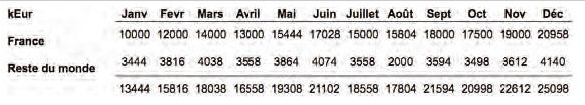
\includegraphics[scale=0.8]{chapitre1/tableau.png}
% 		\caption{  Évolution du chiffre d’affaires par région.} 
% 	\end{center} 
% \end{figure}

% \textit{Mais si nous représentons les séries de chiffres sous forme graphique (ci-dessous),on comprend en un coup d’œil que le chiffre d’affaires ”France” progresse et que le chiffre d’affaires ”Reste du monde” stagne.}

% \begin{figure}[ht] 
% 	\begin{center}
% 		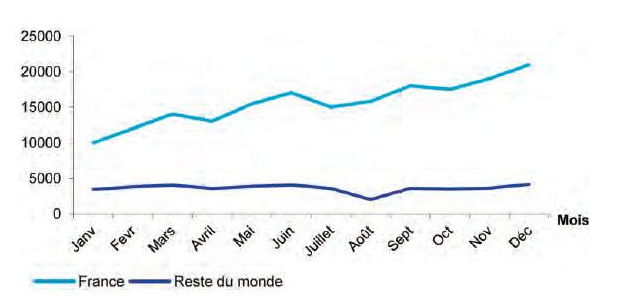
\includegraphics[scale=0.6]{chapitre1/visuatab.png}
% 		\caption{  Évolution du chiffre d’affaires par région.} 
% 	\end{center} 
% \end{figure}



% \leftskip=0cm
% \item\textbf{Vulnérabilité } Vulnerability :\\
		

% Le Big Data apporte de nouveaux problèmes de sécurité. Malheureusement, il y a quotidiennement des violations de données massives.\\

% \leftskip=0,5cm
% \emph{\textbf{Exemple:}}\emph{Rapporté par CRN\footnote{CRN, anciennement Computer Reseller News, est un magazine commercial américain traitant }\blfootnote{d'informatique. Il cible principalement le milieu de la revente informatique}: en mai 2016, “un pirate informatique appelé Peace a posté des données sur le web sombre pour les vendre, qui auraient inclus des informations sur 167 millions de comptes LinkedIn et 360 millions d’e-mails et de mots de passe pour les utilisateurs de MySpace\footnote{Myspace est un site web de réseautage social fondé aux États-Unis en août 2003, qui met }\blfootnote{ gratuitement à disposition de ses membres enregistrés un espace web personnalisé, permettant de }\blfootnote{ présenter diverses informations personnelles et d'y faire un blog} ”\cite{le-datascientist}.}\\

% \end{enumerate}
% \leftskip=0cm
% \textbf{Remarque :} Il existe d’autres sources qui parlent de 54 Vs pour les caractéristiques du Big Data tel que la \textbf{venue} (le lieu), \textbf{valence}, \textbf{vocabulaire}, \textbf{vagueness} (imprécision) ...etc .\newpage

% %Section----------------- Les technologies du Big Data ---------------------
% \section{Les technologies du Big Data}


% Le développement d'applications Big Data est devenu de plus en plus important ces dernières années. En fait, plusieurs organisations de différents secteurs dépendent de plus en plus des connaissances extraites d'énormes volumes de données. Cependant, dans le contexte du Big Data, les techniques et plateformes de données traditionnelles sont moins efficaces. Ils montrent une réactivité lente et un manque d'évolutivité, de performances et de précision. Pour faire face aux défis complexes du Big Data, plusieurs technologies ont été développées pour répondre à plusieurs problématiques comme l’analyse prédictive plus particulièrement dans le cadre de maintenance préventive ou encore de prédiction des ventes et gestion des stocks. L’analyse des données en temps réel est aussi une des applications du Big Data \cite{saagie}.\\






% Nous décrivons ici tous les composants qui font partie des solutions Big Data sous de nombreux angles: matériel, méthodologies, logiciels et applications de base, etc.\\
% Pour mieux catégoriser ces concepts, nous les avons a répartis en différentes sections selon l'objectif visé par chacun. Ces catégories sont: l'\textbf{infrastructure}, le \textbf{stockage}, le \textbf{traitement} et les \textbf{composants de haut niveau}.



% %-------Subsection----------------- Infrastructure ---------
% \leftskip=1cm
% \subsection{Les Infrastructures}

% Le développement du Big Data commence avec les \textbf{cluster Big Data\footnote{Un cluster Big Data est un type spécial de cluster de calcul conçu spécifiquement pour stocker et analyser d’énormes quantités de données non structurées dans un environnement informatique distribué.}}  qui exécutent en parallèle les instructions d'un logiciel de haut niveau. Le cluster est partitionné en deux types de nœuds selon la fonction principale exercée \cite{garcia2016big}: \\


% \begin{itemize}\renewcommand{\labelitemi}{$\bullet$}
%   \leftskip=1,5cm
%   \item Nœuds de données ou esclaves (informatique).
% 	\item Nœuds de gestion ou maîtres (gestion).\\
% \end{itemize}

% \leftskip=1cm
% Outre leurs fonction, le maître et les esclaves peuvent être différenciés par leurs capacités de calcul et leur quantité dans le champ de nœuds.\\

% Les esclaves sont chargés de surveiller les données partitionnées, de traiter et d'interroger les données locales. Les unités de données et de traitement doivent être aussi proches que possible pour éviter les retards introduits par les mouvements entre les partitions. Les nœuds de données sont gourmands en disque et standard en termes de capacités de calcul et de mémoire.\\

% Les maîtres reçoivent et transforment les programmes des applications clientes en instructions parallèles qui peuvent être comprises par les esclaves. Une fois que les applications clientes ont atteint le démon maître, elles finissent par démarrer ou réveiller plusieurs processus dans les esclaves qui retournent finalement une sortie suivant la direction opposée. Parmi l'ensemble des responsabilités approuvées pour les nœuds de gestion figurent: 


% \begin{itemize}\renewcommand{\labelitemi}{$\bullet$}
% \leftskip=1,5cm
% 	  \item La récupération après défaillance.
% 	\item La gestion des ressources.
% 	\item La planification des travaux.
% 	\item La surveillance ou la sécurité.\\
% \end{itemize}

% \leftskip=1cm
% Pour accomplir ces tâches, les maîtres nécessitent une puissance de calcul et de mémoire élevée. Dans les clusters Big Data standard, il suffit de garder deux maîtres support qui se surveillent mutuellement.\\

% Les deux types de nœuds sont connectés via une connexion réseau, généralement LAN (Ethernet ou InfiniBand). Certaines configurations permettent également de connecter les maîtres de différents centres de données sur un réseau WAN pour éviter facilement les défaillances du système. Dans chaque centre de données, le maître et les esclaves sont interconnectés en privé pour ingérer des données, déplacer des données entre les nœuds et effectuer des requêtes. Il existe également un autre réseau public qui sert de façade entre le client et le service de gestion (ssh, VNC, interface web, … ).


% %----------Subsection----------------- Les technologies de Stockage ---------
% \leftskip=1cm
% \subsection{La technologie de Stockage: Le Cloud Computing}

% La plupart des systèmes Big Data reposent sur l'idée d'introduire d'abord des données dans le système sans dépenser trop d'efforts, puis imposer un schéma («schéma en lecture») une fois que les données sont accédées ou traitées. Ce modèle est beaucoup plus polyvalent que celui mis en œuvre par les bases de données relationnel, car le «schéma en lecture» est peu affecté par les mises à jour constantes, généralement présentes dans les systèmes dynamiques actuels des entreprises et des sciences. Dans ce qui suit nous verrons, les technologies de stockage, portées plus particulièrement par le déploiement du \textbf{Cloud Computing}.\\


% Jusqu’ici nous avons bien vu qu’avec le Big Data, les sources de données de plus en plus hétérogènes et localisées sur Internet sont produites de façon continue et à un rythme soutenu. Plusieurs nouvelles solutions ont vu le jour pour traiter ces volumes d’informations et ces flux de données en hausse constante, toutes ces solutions reposent sur un stockage distribué (partitionné) des données sur des clusters\footnote{Un cluster est une grappe de serveurs sur un réseau, appelé ferme ou grille de calcul.}.

% 		\subsubsection{Définitions } 
% 		Plusieurs définitions sont apparus pour décrire cet espace de stockage immense qui n’est tout autre que le cloud computing :\\
% 		%------ BeginEnumerate 2 ------
%     \begin{enumerate}\renewcommand{\theenumi }{\alph{enumi}}
		
% 				\item{\textbf{Définition 1.}}\\
%  		Le "Cloud computing" en français "Informatique dans les nuages" ou "infonuagique" représente des ressources informatiques quelques part en dehors du réseau propre à l’entreprise ou à un particulier autrement dit c'est un concept d’organisation informatique qui place Internet au cœur de l’activité des entreprises, il permet d’utiliser des ressources matérielles distantes pour créer des services accessibles en ligne, L'accès au ressources se fait le plus souvent à l'aide d'un navigateur Web. En une phrase c'est une nouvelle façon de délivrer les ressources informatiques et ça, n'importe où dans le monde \cite{memoirebedjaia}.\\


%         \item{\textbf{Définition 2.}}\\
% C’est un terme général employé pour désigner la livraison de ressources et de services à la demande par Internet. Il désigne le stockage et l’accès aux données par l’intermédiaire d’Internet plutôt que via le disque dur d’un ordinateur. Il s’oppose ainsi à la notion de stockage local, consistant à entreposer des données ou à lancer des programmes depuis le disque dur \cite{avantage-bigdata}.\\


%         \item{\textbf{Définition 3.}}\\ 
% Un paradigme de calcul distribué émergeant dans lequel les données et les services sont disponibles dans des data centers extensibles et peuvent être accédés de manière transparente depuis des appareils (ordinateurs, téléphones, grappes, ...) connectés par Internet \cite{Calcule}. \\


%     \leftskip=1cm
% 	  \textbf{Remarque:}
% 	  \emph{La notion de Cloud ne doit pas non plus être confondue avec celle du NAS\footnote{Network Attached Storage est un serveur de fichiers autonome, relié à un réseau, dont la principale fonction est le stockage de données en un volume centralisé pour des clients réseau hétérogènes.Cette espace est offert pour l'ensemble du réseau local.}, utilisée par beaucoup d’entreprises via un serveur en résidence. Ces réseaux locaux n’entrent pas dans la définition du Cloud. Cependant, certains NAS permettent d’accéder aux données à distance depuis Internet. \cite{avantage-bigdata}}\\

  
	
% \leftskip=0cm
% De manière générale, on parle de Cloud Computing lorsqu’il est possible d’accéder à des données ou à des programmes depuis internet, ou tout du moins lorsque ces données sont synchronisées avec d’autres informations sur Internet. Il suffit donc pour y accéder de bénéficier d’une connexion internet.\\



%  %------ EndEnumerate 2 ------
%  \end{enumerate}

	
	 
% 	\subsubsection{Les caractéristiques du Cloud:}
% 	Selon le \textbf{NIST\footnote{Le National Institute of Standards and Technology, ou NIST (qu'on pourrait traduire par « Institut national des normes et de la technologie »), est une agence du département du Commerce des États-Unis. Son but est de promouvoir l'économie en développant des technologies, la métrologie et des standards de concert avec l'industrie. Cette agence a pris la suite en 1988 du National Bureau of Standards fondé en 1901 avec substantiellement les mêmes missions.}}, le cloud computing doit posséder 5 caractéristiques essentielles qui sont :
		
% 	   \begin{itemize}[label=\textbullet]
	   

% 	    	\item{\textbf{Accès réseau universel:}} L’ensemble des ressources doit être accessible et à disposition de
% l’utilisateur universellement et simplement à travers le réseau.

%         \item{\textbf{Libre service à la demande:}} Permet à l’utilisateur d’utiliser et de libérer des ressources
% distantes en temps réel en fonction des ses besoins, sans nécessiter d’intervention humaine du côté fournisseur.

%         \item{\textbf{Ressources partagées:}} Les ressources matérielles du fournisseur sont partagées entre
% les différents utilisateurs.

%         \item{\textbf{Élasticité:}} Les ressources allouées aux utilisateurs peuvent être augmentées ou diminuées selon l’usage.

%         \item{\textbf{Service mesurable et facturable (pay-as-you-use):}} Les utilisateurs paieront pour les ressources qu’ils ont utilisées et pour la durée de leur utilisation.

% 	   \end{itemize}
			

% \subsubsection{Les services Cloud :}
	
% Selon le type de ressource offerte aux utilisateurs, les services cloud ont tendance à être regroupés selon les trois modèles de base suivants: 
% %------------------------ BeginItemize1 ----------------
% \begin{itemize}\renewcommand{\labelitemi}{$\bullet$}
%   \item Logiciel en tant que service \textbf{(SaaS)}.
% 	\item Plate-forme en tant que service \textbf{(PaaS)}.
% 	\item Infrastructure en tant que service \textbf{(IaaS)} .\\
% \end{itemize}
% %------------------------ EndItemize1 ----------------



% %_____________________________________ figure 1.5____________
% \begin{figure}[H]
% 			 \centering
% 			 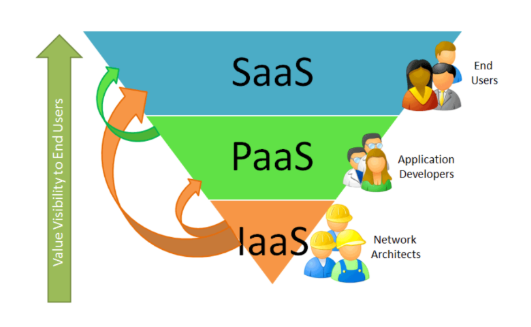
\includegraphics[scale=0.9]{chapitre1/5-ServicesCloud.PNG}
% 			 \caption{Services cloud}
% 			\end{figure}
% %____________________________________________________________

	
%  Dans le prolongement de cette classification, lorsque le service fait référence à une base de données, le modèle est appelé Database as a Service (DBaaS) \cite{campelo2020brief}.\\
 
%  On retrouve dans le tableau suivant TABLE 1.1 les définitions de ces services ainsi que quelques exemple.
% \begin{table}[H]

% \begin{center}

% \footnotesize %taille plus petit que small

% \begin{tabular}{|F{2.5cm}|R{6cm}|R{5cm}|}
% \hline
% \textbf{Service}  & \makecell[c]{\textbf{Définition}} & \makecell[c]{\textbf{Exemple}}\\
% \hline
% IaaS (Infrastructure as a service) &    Fourni a l'entreprise différents composants informatiques comme des espaces de stockages, équipements réseaux, des unités centrales, etc…

% Ce service offre un accès à un parc informatique virtualisé ainsi que des machines virtuelles sur lesquelles l’utilisateur peut installer un système d'exploitation et des applications.
% & \begin{itemize}\renewcommand{\labelitemi}{$\bullet$}
	
% 	\item Amazon EC2 Elastic Compute Cloud.
% 	\item S3 / Simple Storage Service d’Amazon.
% 	\item Google drive, DropBox qui sont gratuits.
% \end{itemize} \\
% %------------------------ EndItemize3 ----------------
% \hline
% PaaS (Platform as a service) & 	Il s’agit d’offrir aux utilisateurs des ressources machines , de l’espace de stockage et une plateforme de développement d’application. Ces plateformes sont spécifiques à un langage et à une base de données, et le système d'exploitation et les outils d'infrastructure sont sous la responsabilité du fournisseur. &  \begin{itemize}\renewcommand{\labelitemi}{$\bullet$}
	
% 	\item App Engine de Google qui se limite à Java et Python.
% 	\item Windows Azure de Microsoft permet de travailler avec les langages comme .NET, PHP, Python, Ruby et Java.
% \end{itemize} \\
% \hline
% SaaS (Software as a Service ) &	Ce service, met des applications à la disposition des utilisateurs. Ces applications peuvent être manipulées à l’aide d’un navigateur web. 

% L’utilisation des applications reste transparente pour les utilisateurs, qui ne se soucient ni de la plateforme, ni du matériels et ni des mise à jour. &   \begin{itemize}\renewcommand{\labelitemi}{$\bullet$}
	
% 	\item Google apps avec Google Docs, Calendar et Gmail qui sont gratuites.
% 	\item Facebook, Linkdin qui sont gratuits.
% 	\item Offices 365 de Microsoft propose des applications web (Word,Excel, PowerPoint, Publisher...).
% \end{itemize} \\
% \hline

% DBaaS (DataBase as a service ) & Un tel modèle fournit des mécanismes transparents pour créer, stocker, accéder et mettre à jour des bases de données. De plus, le fournisseur de services de base de données assume l'entière responsabilité de l'administration de la base de données, garantissant ainsi la sauvegarde, la réorganisation et les mises à jour de version.
% L'utilisation de ce service permet aux fournisseurs de répliquer et de personnaliser leurs données sur plusieurs serveurs, qui peuvent être physiquement séparé [16]. 					
% & \begin{itemize}\renewcommand{\labelitemi}{$\bullet$}
% 	\item Amazon Web Services.
% 	\item RackSpace.
% 	\item IBM, Microsoft, Oracle.  
% 	\end{itemize}
% \\					\hline
% \end{tabular}	
% \caption{Les services Cloud.}
% 	\end{center}
% \end{table}	


%      \emph{\textbf{Remarque:} } \emph{Avec le SaaS on utilise une application, avec le PaaS on construit ses applications et l’IaaS permet d’héberger le tout}.	

			
%   \subsubsection{Les composants clés du cloud computing:}
% 	Le cloud computing est étroitement lié aux mégadonnées. Les composants clés de l'informatique en nuage sont illustrés à la \textbf{Figure 1.6}. Les mégadonnées font l'objet d'une opération à forte intensité de calcul et mettent l'accent sur la capacité de stockage d'un système en nuage. L'objectif principal du cloud computing est d'utiliser d'énormes ressources informatiques et de stockage sous une gestion concentrée, afin de fournir aux applications Big Data une capacité de calcul finie. D'autre part, l'émergence du Big Data accélère également le développement du cloud computing. La technologie de stockage distribué basée sur le cloud computing peut gérer efficacement les Big Data; la capacité de calcul parallèle et améliorer l'efficacité de l'acquisition et de l'analyse des mégadonnées.\\

			
% 			%_____________________________________ figure 1.6____________
%       \begin{figure}[H]
% 			 \centering
% 			 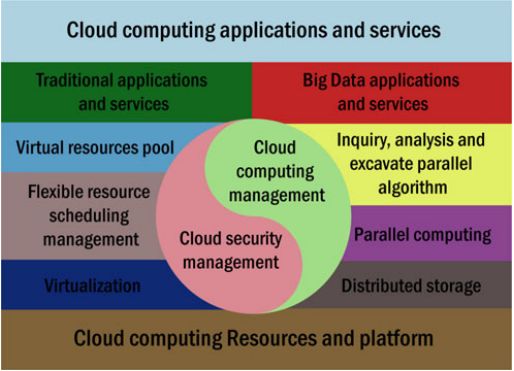
\includegraphics[scale=0.7]{chapitre1/6-ComposantDuCloudComputing.PNG}
% 			 \caption{Composants clés du cloud computing}
% 			\end{figure}
% 			%____________________________________________________________
			
			
	
% Pour comprendre le fonctionnement du Cloud, il faut connaitre ses deux composants à savoir la notion de  Virtualisation et de Data center.\\



% %------ BeginEnumerate 4 ------
% \begin{enumerate}\renewcommand{\theenumi }{\alph{enumi}}

% \item{\textbf{Virtualisation:}}


  			
			
%  C’est l'ensemble des techniques matérielles et/ou logiciels qui permettent de faire fonctionner sur une seule machine, plusieurs systèmes d'exploitation (appelées machines virtuelles (VM), ou encore OS invité).\\

% Même s’il existe plusieurs types de virtualisation, la forme la plus populaire de virtualisation dans le cloud est la virtualisation des serveurs qui consiste à dématérialiser le comportement et les données d’un serveur ou d’une machine, de façon à faire tourner plusieurs de ces instances dématérialisées sur un même serveur physique. De cette façon, les différentes instances créées se partagent les ressources du serveur physique. Cela permet une plus grande modularité dans la répartition des charges, une facilité dans l’administration des serveurs et une réduction des coûts \cite{Ivision}.\\

%     %_____________________________________ figure 1.7____________
%       \begin{figure}[H]
% 			 \centering
% 			 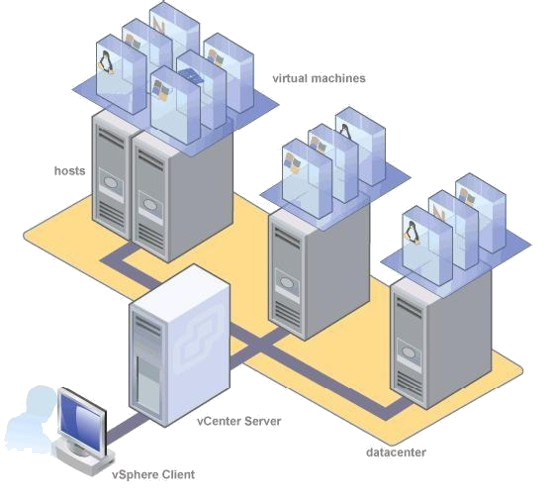
\includegraphics[scale=0.4]{chapitre1/7-VirtualisationDesServeurs.PNG}
% 			 \caption{Virtualisation De Serveurs}
% 			\end{figure}
% 			%____________________________________________________________
			
% \newpage

%   \item{\textbf{Les Data Center:}}


% Un data center ou centre de données, c’est un site physique qui a une infrastructure composée d’un réseau d’ordinateurs et d’espaces de stockage,Il peut être interne ou externe à l’entreprise. Ces sites sont des salle remplies de baies de stockage, utilisées par de nombreuses entreprises et autres organisations gouvernementales \cite{def-data-center}.\\
%  \begin{itemize}
% \item [$\bullet$]\textbf{ Les composants du Data Center :}
% Un centre de données basique regroupe des serveurs, des sous-systèmes de stockage, des commutateurs de réseau, des routeurs, des firewalls, et bien entendu des câbles et des racks physiques permettant d’organiser et d’interconnecter tout cet équipement informatique.

%       %_____________________________________ figure 1.8____________
%       \begin{figure}[H]
% 			 \centering
% 			 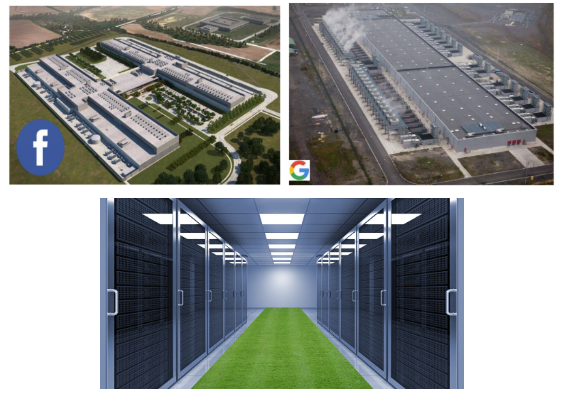
\includegraphics[width=4.7in,scale=1,height=3in]{chapitre1/8-DataCenter.PNG}
% 			 \caption{Exemple de deux data center, un de Facebook et l'autre de Google}
% 			\end{figure}
% 			%____________________________________________________________
			
			
			
		

%       \item [$\bullet$]\textbf{L'architecture du data center}
			
		
			
% 			Théoriquement, n’importe quel espace suffisamment vaste peut servir de Data Center. Cependant, le design et l’implémentation d’un data center nécessite de prendre plusieurs précautions. Par-delà les problèmes basiques du coût et des taxes, les sites sont sélectionnés sur de nombreux critères, comme la localisation géographique, la stabilité météorologique, l’accès aux routes et aux aéroports, la disponibilité énergétique, les télécommunications ou encore l’environnement politique.\\

% Pour fonctionner correctement, un Data Center doit aussi abriter l’infrastructure adéquate : un système distribution d’énergie, un commutateur électriques, des réserves d’énergie, des générateurs dédiés au backup, un système de ventilation et de refroidissement, et une puissante connexion internet. Une telle infrastructure nécessite un espace physique suffisamment vaste et sécurisé pour contenir tout cet équipement.\\

% 	%_____________________________________ figure 1.9____________
% 			\begin{figure}[H]
% 			 \centering
% 			 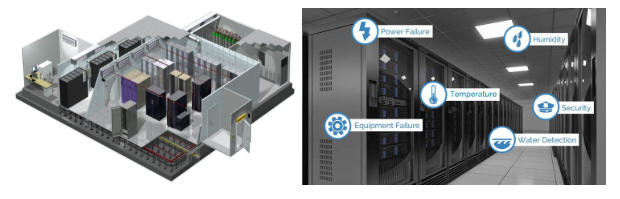
\includegraphics[width=5.5in,scale=1,height=2in]{chapitre1/10-architectureDataCenter.PNG}
% 			 \caption{Architecture des Data Cente}
% 			\end{figure}
% 			%____________________________________________________________
% 			\end{itemize}
% %------ EndEnumerate 4 ------
% \end{enumerate}



% \subsubsection{Les modes et type de stockage dans le Cloud}
%         Le stockage dans le cloud englobe l'archivage, l'organisation et la distribution de données à la demande entre plusieurs volumes de stockage virtualisés, regroupés à partir d'équipements matériels physiques distincts. Plus simplement, le stockage dans le cloud est l'organisation des données stockées dans un emplacement accessible depuis Internet par toute personne qui dispose d'une autorisation \cite{redhat}.\\
				
% 		Le stockage interne présente de nombreuses faiblesses, comme le risque de perdre des données. De plus, le cloud permet de partager très facilement des documents ou des fichiers multimédias trop larges pour être envoyés par mail.\\

% Il existe\textbf{ trois types de stockage} dans le cloud pour les entreprises : 
% \begin{enumerate}
% \leftskip=2cm \item Stockage dans le cloud public.
% \leftskip=2cm \item Stockage dans le cloud privé.
% \leftskip=2cm \item Stockage dans le cloud hybride.\\
% \end{enumerate}

%  En parallèle, il existe trois formats de stockage : 
% \begin{enumerate}
% \leftskip=2cm \item Mode bloc
% \leftskip=2cm \item Mode fichier
% \leftskip=2cm \item Mode objet.\\
% \end{enumerate}
% \textbf{Remarque :} 
%  Chaque format présente ses avantages et ses inconvénients (les blocs sont plus rapides, les fichiers plus lisibles et les objets plus adaptés aux applications cloud-native et mises en paquet dans des conteneurs), mais certains produits de stockage logiciel dans le cloud sont capables de combiner les trois formats dans une solution unique et facile à déployer.

% %------ BeginEnumerate 5 ------
% \begin{enumerate}\renewcommand{\theenumi }{\alph{enumi}}

%     \item \textbf{Les formats de stockage dans le cloud:}\\
    
% Les trois formats de stockage de données dans le cloud :\newpage    
% \begin{itemize}\renewcommand{\labelitemi}{$\bullet$}
%       \item \textbf{Stockage en mode bloc:}\\
      			
% Le stockage en mode bloc permet de diviser un seul volume de stockage (par exemple, un nœud de stockage dans le cloud) en plusieurs instances individuelles appelées blocs. Il s'agit d'une solution de stockage rapide à faible latence, idéale pour les charges de travail hautes performances \cite{redhat}. \\

          
% 					%_____________________________________ figure 1.10____________
% 					\begin{figure}[H]
% 					 \centering
% 					 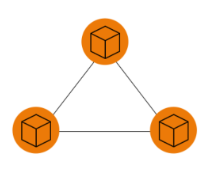
\includegraphics[width=2.5in,scale=1,height=1.6in]{chapitre1/11-StockageEnModeBloc.PNG}
% 					 \caption{Stockage en mode bloc}
% 					\end{figure}
% 					%_____________________________________________________________
					
% 				   \item \textbf{Stockage en mode objet:}\\

% Le stockage en mode objet implique d'attribuer à chaque donnée des identifiants uniques, que l'on appelle les métadonnées. Compte tenu du fait que les objets ne sont ni compensés ni chiffrés, ils sont rapidement accessibles à très grande échelle. Il s'agit donc d'une solution idéale pour les applications cloud-native [19].
%           %_____________________________________ figure 1.11____________
% 					\begin{figure}[H]
% 					 \centering
% 					 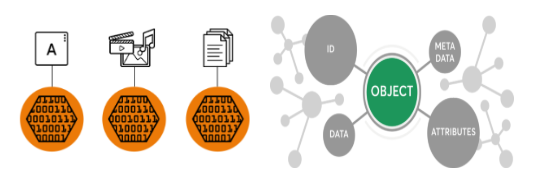
\includegraphics[width=5.5in,scale=1,height=1.7in]{chapitre1/12-StockageEnModeObjet.PNG}
% 					 \caption{Stockage en mode objet}
% 					\end{figure}
% 					%_____________________________________________________________
					
					
%    \item \textbf{Stockage en mode  fichier:}\\

% Le stockage en mode fichier est le plus utilisé sur les systèmes NAS. Il permet d'organiser les données et de les présenter aux utilisateurs. Sa structure hiérarchique permet de parcourir les données du haut vers le bas en toute simplicité, mais augmente le temps de traitement \cite{redhat}.\\
%           %_____________________________________ figure 1.12____________
% 					\begin{figure}[H]
% 					 \centering
% 					 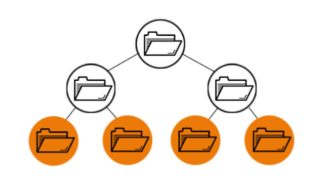
\includegraphics[width=2.5in,scale=1,height=1.6in]{chapitre1/13-StockageEnModeFichier.PNG}
% 					 \caption{Stockage en mode fichier}
% 					\end{figure}
% 					%_____________________________________________________________
					
				
% \end{itemize}



		
			


% \item \textbf{Les types de stockage dans le cloud:}\\

% Il existe trois types de stockage de données dans le cloud :
%     %_____________________________________ figure 1.13____________
% 		\begin{figure}[H]
% 			 \centering
% 			 
\includegraphics[width=5.5in,scale=1,height=2in]{chapitre1/14-TypeDeStockageDansLeCloud.PNG}
% 			 \caption{Type de stockage dans le cloud}
% 		\end{figure}
% 		%_____________________________________________________________
			
			
% 		\begin{itemize}\renewcommand{\labelitemi}{$\bullet$}
% 		  \item \textbf{Stockage dans le cloud public:} \\
			
% Il s'agit du stockage de données entre plusieurs pools de ressources virtuelles nommés clouds publics. Ceux-ci sont développés à partir de matériel détenu et géré par des entreprises tierces. Il n'est pas sans risque de stocker des données dans des systèmes qui ne nous appartiennent pas et qu'on ne gère pas. C'est pour cette raison que de nombreuses entreprises utilisent des conteneurs pour transférer des charges de travail et des applications entre les environnements de cloud public.\\


%     \item \textbf{Stockage dans le cloud prive:} \\
		
% 		Il s'agit du stockage de données entre plusieurs pools de ressources virtuelles nommés clouds privés. Ceux-ci sont alimentés en données par des systèmes dédiés qui sont détenus et gérés par l'entreprise qui les utilise. À long terme, la mise en place manuelle d'un cloud privé à l'échelle de l'entreprise peut se révéler moins efficace que l'utilisation d'un logiciel existant. C'est pour cette raison que les entreprises utilisent des plateformes telles qu'OpenStack\footnote{OpenStack est un ensemble de logiciels open source permettant de déployer des infrastructures de cloud computing (infrastructure en tant que service)} pour réaliser la transformation numérique de leurs pools de ressources virtuelles en clouds privés. \\

% 		\item \textbf{Stockage dans le cloud hybride:} \\
		
% 		Il s'agit du stockage de données dans plusieurs environnements de cloud public et privé, connectés entre eux. Bien que les environnements de cloud privé et public qui composent le cloud hybride restent des entités distinctes, la migration de données entre les deux est facilitée par un réseau complexe de LAN, WPN, API, VPN ou conteneurs. Cette architecture, à la fois séparée et connectée, permet aux entreprises de stocker les données critiques dans leur cloud privé et les données moins sensibles dans le cloud public, tout en les déplaçant entre les différents environnements, selon les besoins.\\
		
% \end{itemize}			

% 		\leftskip= 1cm
% 		\emph{\textbf{Remarque}}
% 		      \emph{La frontière entre le Local Computing et le Cloud Computing est parfois très fine. Pour cause, le Cloud est désormais ancré dans presque toutes les tâches que nous accomplissons sur ordinateur. }\\
		
% %------ EndEnumerate 5 ------
% \end{enumerate}



% %------ EndEnumerate 1 ------







% %----------Subsection----------------- Les technologies de traitement ---------
% \leftskip=1cm
% \subsection{Les technologies de traitement}

% Dans cette section nous parlerons de l’arrivée des technologies de traitement ajustées, plus spécialement sur la mise au point de modes de calcul à haute performance ( MapReduce ), nous parlerons de ( Hadoop ) une solution de big data très largement utilisée pour effectuer des analyses sur de très grands nombres de données, et enfin nous clôturons cette section avec le développement de nouvelles bases de données adaptées aux données non structurées (NoSQL) et nous verrons qu’est se que le NewSQL \cite{businessIntelligence}.\\
		
		
		
% 		%------ BeginEnumerate 6 ------
% 		\begin{enumerate}
		
		
% 		     \item \textbf{Hadoop:} \\
% 				  Hadoop est un framework logiciel open source permettant de stocker des données, et de lancer des applications sur des grappes ( cluster ) de machines standards. Cette solution offre un espace de stockage massif pour tous les types de données, une immense puissance de traitement et la possibilité de prendre en charge une quantité de tâches virtuellement illimitée. Basé sur Java, ce framework fait partie du projet Apache, sponsorisé par Apache Software Foundation.\\
					
% 					Grâce au framework MapReduce, il permet de traiter les immenses quantités de données. Plutôt que de devoir déplacer les données vers un réseau pour procéder au traitement, MapReduce permet de déplacer directement le logiciel de traitement vers les données.\newpage

% Dans son principe, Hadoop se compose essentiellement de : \\


%            %_____________________________________ figure 1.14____________
% 					 \begin{figure}[H]
% 						 \centering
% 						 
\includegraphics[scale=0.5]{chapitre1/15-LesComposantdHadoop.PNG}
% 						 \caption{Les composants d'Hadoop.}
% 						\end{figure}
% 						%____________________________________________________________
						


%       %------ BeginEnumerate 7 ------
% 		  \begin{enumerate}\renewcommand{\theenumi }{\alph{enumi}}
			
%            \item{\textbf{Système de gestion de fichiers HDFS:}} (Hadoop Distributed File System)\\
					
%  		HDFS est est un système de fichiers distribué, extensible et portable Inspiré par GFS\footnote{(Google file system) un système de fichier distribué conçu par Google} et écrit en Java. Il est conçu pour être un système de stockage distribué, évolutif et résilient, conçu pour interagir facilement avec MapReduce. Il fournit une bande passante d’agrégation importante tout au long du réseau. Comme pour GFS, un réseau HDFS est composé d’un nœud maître appelé Namenode et des serveurs de données appelés Datanodes, comme expliqué dans la \textbf{Figure 5}. La structure du fichier HDFS est divisée en blocks d'octets de grande taille par défaut 64 Mo  pour optimiser les temps de transfert et d'accès. Il est toutefois possible de monter à 128 Mo, 256 Mo, 512 Mo voire 1 Go\cite{mapreduce}.\\ \\
% Ces blocs sont ensuite répartis sur plusieurs machines, permettant ainsi de traiter un même fichier en parallèle. Pour garantir une tolérance aux pannes, les blocs de chaque fichier sont répliqués sur plusieurs machines. Notez que si la taille du fichier est inférieure à la taille d’un
% bloc, le fichier n’occupera pas la taille totale de ce bloc.


         
% 				  %_____________________________________ figure 1.15____________
% 					\begin{figure}[H]
% 					 \centering
% 					 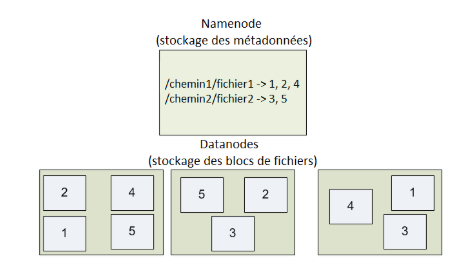
\includegraphics[width=5.5in,scale=1,height=3in]{chapitre1/16-Architecture HDFS.PNG}
% 					 \caption{Architecture HDFS.}
% 					\end{figure}
% 					%_____________________________________________________________
					
					

% \newpage
%          \item \textbf{Modèle de programmation Map-reduce:} \\

% Le framework MapReduce permet de traiter les immenses quantités de données. Plutôt que de devoir déplacer les données vers un réseau pour procéder au traitement, MapReduce permet de déplacer directement le logiciel de traitement vers les données. Ce modèle fera l’objet de la deuxième technologie que nous allons présenter.\\

%         \item  Une collection d’outils spécifiques pour HDFS et Map Reduce comme des API et des frameworks.\\


     
%     \end{enumerate}
% 		%------ EndEnumerate 7 ------
				
%   \item \textbf{Map-reduce:} MapReduce a été introduit par Google et décrit en détails dans la publication \textbf{«MapReduce: Simplified Data Processing on Large Clusters »} publiée en 2004 et ça pour faciliter la mise en œuvre de ses workflows de traitement parallèle. L'objectif principal était de remplacer la programmation complexe et non intuitive sur l'informatique distribuée (préalablement abordée par les plateformes HPC) par une plateforme transparente moderne avec seulement deux fonctions: Map et Reduce. Ces deux fonctions définies par l'utilisateur permettent aux utilisateurs d'utiliser les ressources distribuées sans se plaindre du réseau, de la planification, de la récupération après défaillance, etc.\\

% Un modèle aussi intuitif que le MapReduce ne nécessite pas d’expertise concernant le parallélisme et les systèmes distribués. Son Framework Plug-and-Play embarque tous les détails pour implémenter les systèmes de calcul parallèle, la persistance et la résilience, l’optimisation et l’équilibre des ressources.



%       %_____________________________________ figure 1.16____________
%       \begin{figure}[H]
% 			 \centering
% 			 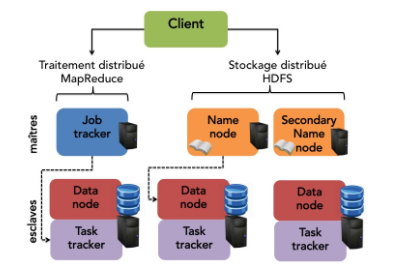
\includegraphics[scale=1]{chapitre1/17-EnvironnementHadoop.PNG}
% 			 \caption{L'environnement Hadoop.}
% 			\end{figure}
% 			%_____________________________________________________________



%       %------ BeginEnumerate 8 ------
% 		  \begin{enumerate}\renewcommand{\theenumi }{\alph{enumi}}
			
%                     \item{ \textbf{Principe de MapReduce:} } \\

% Le Framework se décompose en deux parties. La fonction Map permet aux différents points du cluster distribué de distribuer leur travail. La fonction Reduce permet de réduire la forme finale des résultats des clusters en un seul résultat.Cela est rendu possible grâce au système de fichiers distribués HDFS d’Hadoop.Ce Framework est également constitué de plusieurs composants \cite{top5}:\\

%     	%------------------------ BeginItemize6 ----------------
% 		\begin{itemize}
% 		    \leftskip=1cm
% 				\item[$\bullet$] \textbf{Job tracker :} Est le nœud principal qui gère toutes les tâches et les ressources d’un cluster.
% 				\item[$\bullet$]  \textbf{Les TaskTrackers :} Sont les agents déployés sur chaque machine d’un cluster pour lancer la map et réduire les tâches..
% 				\item[$\bullet$]  \textbf{JobHistoryServer:} est un composant permettant de suivre les tâches complétées, généralement déployé comme une fonction séparée ou avec JobTracker.\\
				
				
% 		\end{itemize}
% 		%------------------------ EndItemize5 ----------------

%      \leftskip=1cm
%      \textbf{Exemple d'utilisation de MapReduce:}  \emph{ Dans ce qui suit on vient mettre en clair le fonctionnement
%      	de MapReduce avec l’exemple typique ”Word Count” schématisé afin de	mieux cerner le rˆole de chaque fonction de ce framework.
%      	\\ s’il est possible de compter manuellement le nombre de fois qu’un mot apparaît dans un roman, cela prend beaucoup de temps. Si l’on répartit cette tâche entre une vingtaine de personnes, les choses peuvent aller beaucoup plus vite. Chaque personne prend une page du roman et écrit le nombre de fois que le mot apparaît sur la page. Il s’agit de la partie Map de MapReduce. Si une personne s’en va, une autre prend sa place. Cet exemple illustre la tolérance aux erreurs de MapReduce. Lorsque toutes les pages sont traitées, les utilisateurs répartissent tous les mots dans 26 boîtes en fonction de la première lettre de chaque mot. Chaque utilisateur prend une boîte, et classe les mots par ordre alphabétique. Le nombre de pages avec le même mot est un exemple de la partie Reduce de MapReduce.}
     
%      \begin{figure}[H]
%      	\centering
%      	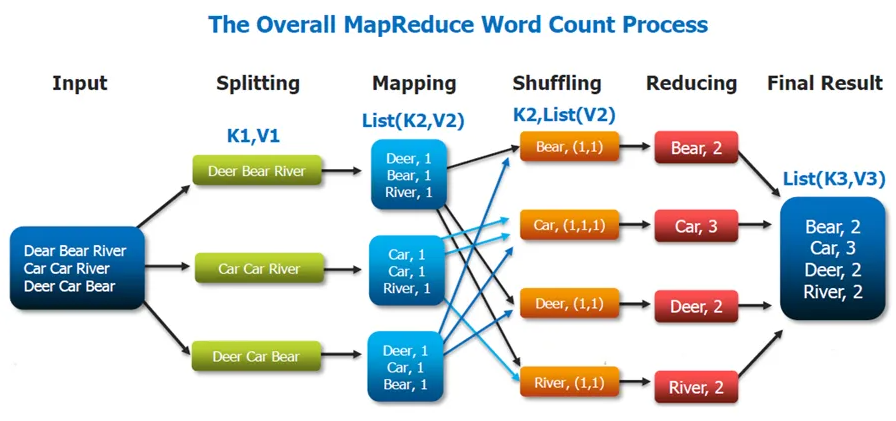
\includegraphics[scale=0.6]{chapitre1/mapred.PNG}
%      	\caption{Exemple de Word Count.}
%      \end{figure}
 
% \newpage

%     \leftskip=1cm
%     \item{ \textbf{Les avantages de MapReduce:} } Parmi les avantages de la programmation MapReduce nous citons:


% %------------------------ BeginItemize7 ----------------
% \begin{itemize}
%     \leftskip=1,5cm
		
%     	\item[$\bullet$]  La scalabilité.
% 		\item[$\bullet$]  La flexibilité.
% 		\item[$\bullet$]  La sécurité et l’authentification.
% 		\item[$\bullet$]  Le traitement parallèle.
% 		\item[$\bullet$]  La disponibilité.
% 		\item[$\bullet$]  Un modèle simple de programmation.\\
% \end{itemize}
% %------------------------ EndItemize7 ----------------



% \end{enumerate}
% %------ EndEnumerate 8 ------


% \leftskip=1cm
% \item  \textbf{Les bases de données NoSQL:} \\
      
% De nos jours, l’ubiquité de la connexion Internet est une réalité (les voitures que nous conduisons, les montres que nous portons, nos petits appareils médicaux domestiques, nos réfrigérateurs et congélateurs, nos Smartphones et ordinateurs portables). De plus, les données numériques produites par les êtres humains, dont les séquences vidéo, les photos et autres, atteignent des volumes importants de plusieurs EO par jour. Ces données actuellement stockées dans des bases qui leur ont été conçues spécifiquement sont gérés par des logiciels de gestion de bases de données volumineuses, jouant le rôle d’intermédiaires entre les bases de données d’un côté et les applicatifs et leurs utilisateurs de l’autre. On parle ici des bases de données non-relationnelles, dites NoSQL.\\

% Concrètement une base de données NoSQL est une approche de la conception des bases et de leur administration particulièrement utile pour de très grands ensembles de données distribuées. Elle englobe une gamme étendue de technologies et d’architectures, afin de résoudre les problèmes de performances en matière d’évolutivité et de Big Data que les bases de données relationnelles ne sont pas conçues pour affronter. De plus elle est particulièrement utile lorsqu’une entreprise doit accéder, à des fins d’analyse, à de grandes quantités de données non structurées ou de données stockées à distance sur plusieurs serveurs virtuels du Cloud.\\

% Pour mieux comprendre les bases de données NoSQL et leur application dans le Big Data, nous consacrons \textit{\textbf{le chapitre 3 "Base de données NoSQL"}} à la description de cette technologie.



%  \end{enumerate}
%  %------ EndEnumerate 6 ------





% %----------Subsection----------------- Moteurs de traitement distribuées ---------
% \leftskip=1cm
% \subsection{Les moteurs de traitement distribuées}

% Les frameworks de traitement distribuée dans le Big Data sont responsables de l'ingestion, du filtrage, de la transformation, de l'apprentissage, de l'interrogation et de l'exportation de grandes quantités de données. Pourtant, il existe de nombreuses implémentations pour ce concept. La plupart des frameworks distribués modernes suivent un schéma d'instructions multiples à plusieurs instructions, afin d'exécuter la même séquence d'instructions simultanément sur un ensemble distribué de partitions de données. En plus de définir le schéma principal d'exécution, ces cadres font également face à d'autres problèmes, tels que le redémarrage des processus ayant échoué, la planification des travaux, la synchronisation du réseau, l'équilibrage de charge, etc \\

% Les modèles les plus pertinents pour les implémentation, actuelles de l’informatique distribuée sont : \\



%       %------ BeginEnumerate 9 ------
% 		  \begin{enumerate}\renewcommand{\theenumi }{\alph{enumi}}
			
       
%           \item{ \textbf{DAG: Traitement parallèle de graphiques acycliques dirigés: } } (Directed Acyclic Graph Parallel Processing)\\ \\
% 				  Tous les frameworks distribués basés sur DAG pour les Big Data, comme Spark\footnote{Spark est un framework open source de calcul distribué. Il s'agit d'un ensemble d'outils et de composants logiciels structurés selon une architecture définie. Développé à l'université de Californie à Berkeley par AMPLab, Spark est aujourd'hui un projet de la fondation Apache.}, organisent leurs tâches en les divisant en un plus petit ensemble de tâches atomiques. Dans ce modèle, les sommets correspondent à des tâches parallèles, tandis que les arêtes sont associées à l'échange d'informations. Comme le montre la \textbf{ figure 1.18 }, les sommets peuvent avoir plusieurs connexions entre les entrées et les sorties, ce qui implique que la même tâche peut être exécutée dans différentes données et les mêmes données dans différentes partitions. Les flux de données sont physiquement pris en charge par la mémoire partagée, les canaux ou les disques. Les instructions sont dupliquées et envoyées du maître aux nœuds esclaves pour une exécution parallèle.
					


% 								 %_____________________________________ figure 1.17____________
% 								 \begin{figure}[H]
% 								 \centering
% 								 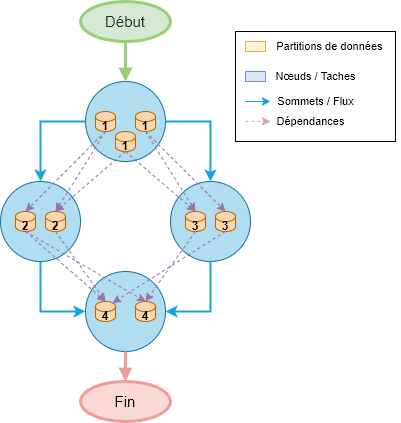
\includegraphics[width=4.5in,scale=1,height=2.7in]{chapitre1/21-DAG.PNG}
% 								 \caption{Traitement parallèle du graphique acyclique direct.}
% 								 \end{figure}
% 								 %_____________________________________________________________

% La \textbf{ figure 1.18 } illustre un programme d'exécution DAG avec 4 tâches et différentes configurations de partition pour chaque tâche. Par exemple, la tâche la plus élevée du graphique est formée de 3 partitions. Une fois cette tâche terminée, deux tâches dépendantes (3 et 4) sont démarrées. Les dépendances entre les partitions ne sont pas triviales comme on peut le voir sur la figure. La partition la plus à droite dans la tâche 2 ne dépend que de deux partitions d'entrée, tandis que les partitions à l'extrême gauche ont une seule dépendance. Enfin, l'entrée de la tâche 4 est liée à la sortie des tâches 2 et 3. Il convient donc de remarquer les différences entre les données (lignes noires en pointillés) et les dépendances des tâches (lignes bleues).\newpage


           
%            \item{ \textbf{BSP: Traitement parallèle synchrone en vrac: } } (Bulk Synchronous Parallel Processing)\\
					
% Les systèmes BSP sont formés par une série de super-étapes connectées, implémentées sous forme de graphiques dirigés. Dans ce schéma, les données d'entrée sont le point de départ. D'ici à la fin, un ensemble de super-étapes est appliqué aux données partitionnées afin d'obtenir la sortie finale. Comme mentionné précédemment, chaque super-étape correspond à un graphe indépendant associé à une sous-tâche à résoudre. Une fois toutes les sous-tâches de composition terminées, la synchronisation en bloc de toutes les sorties est validée. À ce stade, les sommets peuvent envoyer des messages à l'étape suivante, ou en recevoir des étapes précédentes, ainsi que pour modifier son état et ses bords sortants.\\



% 								 %_____________________________________ figure 1.18____________
% 								 \begin{figure}[H]
% 								 \centering
% 								 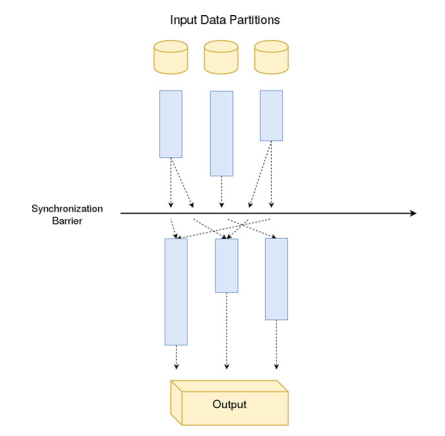
\includegraphics[width=4.5in,scale=1,height=4in]{chapitre1/22-BSP.PNG}
% 								 \caption{Traitement BSP.}
% 								 \end{figure}
% 								 %_____________________________________________________________
								
					
								
% La \textbf{ figure 1.19 } montre un exemple pour le traitement BSP avec deux supersteps et une barrière de synchronisation. Les sous-tâches de chaque super-étape sont représentées sous forme de rectangles de hauteur variable (durée de la tâche) et les flux de données sous forme de lignes en pointillés. La barrière de synchronisation agit comme un proxy temporel entre les étapes. Bien que la sous-tâche ne puisse pas démarrer avant la fin de chaque sous-tâche précédente, la communication entre les étapes est cependant autorisée.

%       \end{enumerate}
%       %------ EndEnumerate 9 ------


% %Section-------------------------------------------- Les sources du big data ----------------------------------------------
% \leftskip=0cm
% \section{Les sources du big data} 


% Pour réussir avec le Big Data, il est important que les entreprises disposent du savoir-faire pour passer en revue les différentes sources de données disponibles et classer en conséquence leur convivialité et leur pertinence \cite{top5}.\\
% \leftskip=0cm
% Deux classifications des sources du Big Data sont donnés dans ce qui suit :

% \begin{enumerate}
% \leftskip=1cm
% \item Selon qu'elles soient interne ou externe à l'entreprise.
% \item Selon leur provenance.\\

% \end{enumerate}




		
		  
	
% 	\leftskip=0cm
% 	\subsection{ Les données internes ou externes à l'entreprise} 
	 
% 		 \leftskip=0cm
% 		 Les données sont internes si une entreprise les génère, les possède et les contrôle .\\ \\
% 		 \textbf{Exemple:}
		
		    
%         %------------------------ BeginItemize8 ----------------
% 				\begin{itemize}
% 			  	\leftskip=1cm
% 				  \item[$\bullet$]  Module ERP d'entreprise.
% 				  \item[$\bullet$]  Capteurs, contrôleurs.
% 				  \item[$\bullet$]  Centres d'appels internes.
% 				  \item[$\bullet$]  Journaux de site Web.\\
% 				\end{itemize}
%         %------------------------ EndItemize8 ----------------

		
% 		\leftskip=0cm
% Les données externes sont des données publiques ou des données générées en dehors de l'entreprise; en conséquence, la société ne la possède ni ne la contrôle .
%      \textbf{Exemple:}
		   
			  
%         %------------------------ BeginItemize9 ----------------
% 				\begin{itemize}
% 			 	  \leftskip=1cm
% 					\item[$\bullet$]  Médias sociaux.
% 					\item[$\bullet$]  Statistiques officielles.
% 					\item[$\bullet$]  Prévisions météorologiques.
% 					\item[$\bullet$]  Ensembles de données accessibles au public pour l'apprentissage automatique.\\
% 				\end{itemize}	
%         %------------------------ EndItemize9 ----------------
        	
		
% 		\subsection{Les sources du big data selon leur provenances :} Les données les plus volumineuse sont utilisées aujourd'hui par les organisations et les entreprises dans le seul but d'effectuer des analyses. Toutefois, avant de pouvoir extraire des informations et des renseignements précieux à partir de données importantes, ces dernières doivent connaître plusieurs sources de données importantes. Les données, comme nous le savons, sont massives et existent sous diverses formes. Si elles ne sont pas bien classées ou si elles ne proviennent pas d'une source sure, elles peuvent finir par faire perdre du temps et des ressources précieuses. Afin de réussir avec les données volumineuses, il est important que les entreprises aient le savoir-faire nécessaire pour faire le tri entre les différentes sources de données disponibles et classer en conséquence leur utilité et leur pertinence.
		
% 		    %_____________________________________ figure 1.19____________
% 		\begin{figure}[H]
%      \centering
%      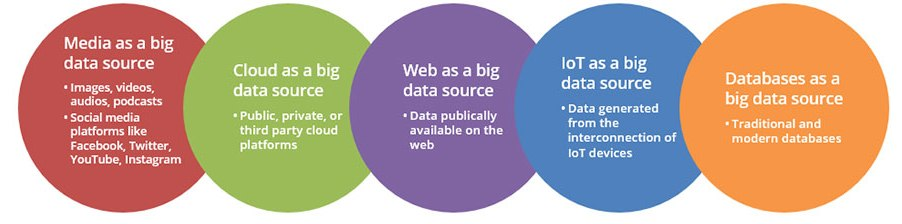
\includegraphics[width=6in,scale=1,height=1.5in]{chapitre1/18-SourcesDuBigData.jpg}
%      \caption{Les 5 sources du Big Data.}
%     \end{figure}
% 		%_____________________________________________________________
		
	
	
			
			
			
			

		
		
		
		
		  
% 			%------ BeginEnumerate 10 ------
		  
			
          
%           \subsubsection{Les médias:} 
% 		Les médias sont la source la plus populaire de mégadonnées, car ils fournissent des informations précieuses sur les préférences des consommateurs et l'évolution des tendances. Ces données sociales  proviennent des mentions J'aime, des tweets et des retweets, des commentaires, des téléchargements de vidéos et des médias généraux qui sont téléchargés et partagés via les plateformes de médias sociaux préférées au monde. Ce type de données fournit des informations inestimables sur le comportement et le sentiment des consommateurs et peut être extrêmement influent dans les analyses marketing.\\
		
	
% 		\emph{\textbf{Exemple : }Les médias comprennent les médias sociaux et les plates-formes interactives, telles que Google, Facebook, Twitter, YouTube, Instagram, ainsi que des supports
% génériques tels que des images, des vidéos, des audios et des podcasts qui fournissent des informations sur l'interaction utilisateur.\\}
   		
% 		      \subsubsection{ Le cloud: }
% Aujourd'hui, avec la croissance accélérée du volume de données utilisé par les applications, de nombreuses organisations ont déplacé leurs données vers des serveurs cloud pour fournir des services évolutifs, fiables et hautement disponibles \cite{futura-tech}.\\

% Le stockage cloud héberge des données structurées et non structurées et fournit aux entreprises des informations en temps réel et des informations à la demande. Le principal attribut du cloud computing est sa flexibilité et son évolutivité. Comme les mégadonnées peuvent être stockées et sourcées sur des clouds publics ou privés, via des réseaux et des serveurs, le cloud constitue une source de données efficace et économique car les ressources sont fournis à la demande et on ne paye que les ressources utilisées \cite{top5}.

% 		      \subsubsection{ Le Web: }
% 		Le Web public constitue une source répandu et facilement accessible pour le Big Data. Les données sur le Web ou «Internet» sont généralement disponibles pour les particuliers et les entreprises. De plus, des services Web tels que Wikipedia fournissent des informations gratuites et rapides à tout le monde. Le Web public est également une autre bonne source de données sociales, et des outils comme Google Trends peuvent être utilisés à bon escient pour augmenter le volume de données.\\
	
% L'énormité du Web garantit sa polyvalence et est particulièrement bénéfique pour les start-ups et les PME, car elles n'ont pas à attendre pour développer leur propre infrastructure et référentiels de Big Data avant de pouvoir tirer parti du Big Data.

%          \subsubsection{ L’Internet Des Objets (IoT): }
% Les données machine sont définies comme des informations générées par des équipements industriels, des capteurs installés dans des machines et même des journaux Web qui suivent le comportement de l'utilisateur. En logistique, il peut s'agir de capteurs qui servent à la traçabilité des biens pour la gestion des stocks et les acheminements.\\
% En domotique, l'IoT recouvre tous les appareils électroménagers communicants, les capteurs , les compteurs intelligents et systèmes de sécurité connectés des appareils de type box domotique. Le phénomène IoT est également très visible dans le domaine de la santé et du bien-être avec le développement des montres connectées, des bracelets connectés et d'autres capteurs surveillant des constantes vitales labrinidis2012challenges].\\

 

% \emph{\textbf{Exemple :} En Tennis, la marque Zepp propose un système de capteur connecté qui analyse vos performances sur le terrain.
% Il suffit de fixer le capteur sur le manche de n’importe quelle raquette de tennis et de se mouvoir pour obtenir un retour d’information instantané sur iPhone, iPad ou appareil Android.  }

%          \subsubsection{ Les bases de données: }
% Les entreprises préfèrent aujourd'hui utiliser une fusion de bases de données traditionnelles et modernes pour acquérir des mégadonnées pertinentes. Cela permet  d’ouvrir la voie à un modèle de données hybride avec un faible coût d'investissement. De plus, ces bases de données sont également déployées à plusieurs fins de Business Intelligence.
% Le processus d'extraction et d'analyse de données parmi de vastes sources de mégadonnées est un processus complexe qui peut être frustrant. Ces complications peuvent être résolues si les organisations englobent toutes les considérations nécessaires des mégadonnées, et prennent en compte les sources de données pertinentes et les déploient d'une manière bien adaptée à leurs objectifs organisationnels.\\


% \emph{\textbf{Exemple :} Les bases de données les plus populaires Microsoft SQL Server, MongoDB, Oracle, MySQL et IBM Db2 ..etc.}


% %------ EndEnumerate 10 ------












% %Section-------------------------------------------- Les nouveaux métiers du Big Data ----------------------------------------------

% \section{Les nouveaux métiers du Big Data} 

% Les emplois Big Data, ou métiers de la donnée, sont de plus en plus nombreux. Les entreprises de tous les secteurs cherchent désormais à exploiter les données à leur disposition pour aiguiller leur stratégie et leur développement.Toutefois, pour être en mesure d’exploiter ces données, les entreprises doivent s’appuyer sur des compétences et du savoir-faire de professionnels hautement qualifiés capables d’utiliser les technologies analytiques. Ainsi, le Big Data a donné naissance à de nombreux nouveaux métiers : Data Miner, Data Analyst, Chief Data Officer, Data Architect, Data Scientist… Ces experts sont en mesure de collecter des données, de les organiser, de les traiter, et de les transformer en informations exploitables par tous les départements de l’entreprise.\\

%     \textbf{Note:} \emph{Selon le Robert Half 2018 Salary Guide for Technology Professionals, les emplois Big Data seront les plus demandés au cours des années à venir. 67 \% des exécutifs d’entreprises affirment que le Big Data est l’un des principaux facteurs de recrutement, au même titre que le marketing numérique et le cloud.}
    
    


%     %_____________________________________ figure 1.21____________
%     \begin{figure}[H]
%      \centering
%      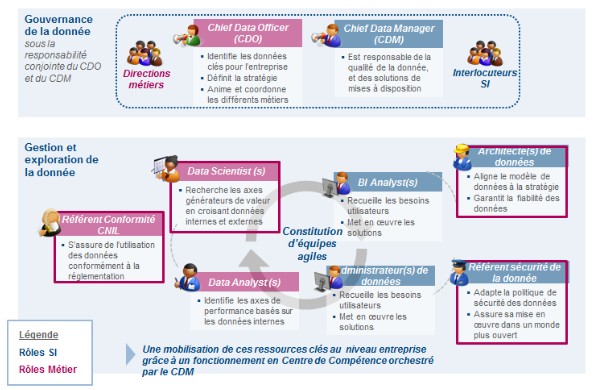
\includegraphics[scale=0.7]{chapitre1/20-EmploisBigData.PNG}
%      \caption{Exemple d'emplois Big Data.}
%     \end{figure}
% 		%_____________________________________________________________

% \begin{table}[H]
% \begin{center}


% \footnotesize
% \begin{tabular}{|F{3cm}|R{9cm}|}
%   \hline
% Métiers & \makecell[c]{Description} \\
%   \hline
%   Chief data officer & Appelée Directeur de données ou bien Directeur de la transformation digitale est l’un des métiers du Big Data, Il cumule de nombreux savoir faire (marketing, stratégie, IT, business, innovation, logique d’entreprise, process) et savoir être (communication, ouverture aux autres, capacités à convaincre. . . ) pour prendre en charge cette fameuse mutation numérique. \\

% \hline 
%   Big Data Architect & Tout comme les architectes créent des structures physiques, les architectes de données élaborent des schémas pour des systèmes de gestion de données. Il s’agit de l’un des métiers du Big Data qui combine les compétences en design et en implémentation de systèmes de gestion de données.
  
% C’est la personne qui se charge de collecter des données brutes pour l’entreprise. Leur quantité peut aussi varier énormément. Après avoir collecté les données brutes, l’architecte Big Data se charge de créer et d’optimiser des infrastructures de stockage, manipulation et restitution. Il doit élaborer une architecture de Data Management et concevoir un plan pour intégrer, centraliser, protéger et maintenir les données. \\
%  \hline
%   Data engineer & L’ingénieur Big Data collabore avec des entreprises pour développer, entretenir, tester et évaluer des solutions Big Data. La plupart du temps, ils utilisent leurs compétences en technologies Hadoop comme MapReduce, HiveMongo DB, ou Cassandra. L’ingénieur Big Data crée des systèmes de traitement de données à grande échelle. Il est également expert en solutions de Data Warehousing et en technologies de bases de données.\\

%   \hline
%   Data scientist & Le Data Scientist est chargé de développer les algorithmes nécessaires pour poser les bonnes questions et obtenir les bonnes réponses afin de tirer des informations pertinentes de vastes ensembles de données. Il est donc nécessaire d’avoir de solides connaissances en statistiques, en mathématiques, en modèles prédictifs et en stratégie d’entreprise.\\

%   \hline
  
%   Data Analyst & Le métier de Data Analyst a commencé à apparaître dans les appels d’offres ces derniers temps car les entreprises ont ressenti le besoin d’avoir les données valorisées et synthétisées sous forme d’indicateurs de performance , et de tableaux de bords. Le Data Analyst aide les entreprises à véritablement consommer les données mis en forme par le Data Engineer ou les résultats renvoyés par les modèles du Data Scientist pour la prise de décision effective. C’est un métier à l’intersection de la Business Intelligence et de l’ingénierie Big Data. Le Data Analyste maîtrise les outils de reporting, de visualisation , l’outil de suivi par excellence des décideurs , la programmation VBA, le SQL, et possède de très bonnes aptitudes communicationnelles pour échanger avec les décideurs de l’entreprise sur la signification des indicateurs calculés sur la base des données.\\

 
%   \hline
%   Data miner & Son rôle assez proche de celui de Data Analyst, il est responsable principalement de la fouille de données.\\

%    \hline
%    Data protection officer & C’est le chef d’orchestre de la conformité. Les responsables le consultent lors du traitement de données à caractère personnel, aussi bien en ce qui concerne la sécurité informatique que la sécurité juridique.\\
%     \hline   


%      Business intelligence manager & Il gère une équipe de développeurs et d’analystes,Ce gestionnaire est dans un premier temps chargé d’identifier les besoins de l’entreprise en matière de Business Intelligence. Il doit analyser les informations pertinentes, et fournir des rapports détaillés basés sur ces analyses pour permettre à l’entreprise d’agir.\\
%      \hline
% \end{tabular}
% \caption{Métiers et description d'emplois dans Big Data.}
% \end{center}
% \end{table}
% \newpage
% %----------------- Conclusion Chapitre 1.1-------------------------
% \section*{Conclusion}
% \leftskip=0,5cm


% Au cours des dernières années un nombre important de sources de données est devenu disponible et à la portée de tous. Le Big Data en tant que discipline a déjà traversé son cycle d'implantation et est aujourd'hui transversal pour toute entreprise axée sur les données. Ainsi, les solutions et technologies Big Data représentent le moyen actuel d'atteindre la compétitivité et la croissance de notre société, où les appareils connectés augmentent rapidement, générant des données à des taux toujours croissants.\\
% Comme nous l'avons vue dans la section 1.7 dans ce chapitre, les sources du Big Data sont nombreuses et varies. On s'intéresse dans le cadre ce travail à l'une des plus grand source du Big Data à savoir l'IoT.\\
% En effet, le volume de données générées par l’Internet des Objets ( IoT ) prend de plus en plus d’ampleur. Ainsi, pour pouvoir les prendre en charge et les analyser en temps réel, il est nécessaire de s’en remettre aux outils analytiques Big Data. C’est la raison principale de la relation étroite entre l’Internet des Objets et le Big Data.\\
% Dans le paradigme IoT, une énorme quantité de capteurs réseau sont intégrés dans divers appareils et machines dans le monde réel. Ces capteurs déployés dans différents domaines peuvent collecter différents types de données, telles que des données environnementales, des données géographiques, des données astronomiques et des données logistiques. Les équipements mobiles, les installations de transport, les installations publiques et les appareils électroménagers pourraient tous être des équipements d'acquisition de données dans l'IoT. Les mégadonnées générées par l'IoT ont des caractéristiques différentes par rapport aux mégadonnées générales en raison des différents types de données collectées , dont les caractéristiques les plus classiques incluent l'hétérogénéité, la variété, la caractéristique non structurée, le bruit et la redondance élevée.\\
% Bien que les données IoT actuelles ne soient pas la partie dominante des mégadonnées, d'ici 2030, la quantité de capteurs atteindra un billion, puis les données IoT seront la partie la plus importante des mégadonnées. Selon de nombreuses études le Big Data dans l'IoT a trois fonctionnalités conformes au paradigme du Big Data:\\






%                  %------ BeginEnumerate 20 ------
%                  \begin{itemize}\renewcommand{\labelitemi}{$\bullet$}

% 				             \item  Des terminaux abondants générant de grandes masses de données.
% 										 \item  Les données générées par l'IoT sont généralement semi-structurées ou non structurées.
% 										 \item  Les données de l'IoT ne sont utiles que lorsqu'elles sont analysées.\\
% 									\end{itemize}	
% 									%------ EndEnumerate 20 ------
										
										
% À l'heure actuelle, de nombreux opérateurs de l'IoT se rendent compte de l'importance des mégadonnées, car le succès de l'IoT repose sur l'intégration efficace des mégadonnées et du cloud computing. Le déploiement généralisé de l'IoT fera également entrer de nombreuses villes dans l'ère des mégadonnées.\\
					
% Aujourd’hui, les objets connectés couplés à la capacité d’analyse du Big Data fournissent aux entreprises, aux particuliers et aux administrations de nouveaux leviers d’action. Il a été largement reconnu que ces deux technologies sont interdépendantes et devraient être développées conjointement: \\
								
										
										
							
%                  %------ BeginEnumerate 21 ------
%                  \begin{itemize}\renewcommand{\labelitemi}{$\bullet$}

% 				             \item  D'une part, le déploiement généralisé de l'IoT stimule la forte croissance des données à la fois en quantité et en catégorie, offrant ainsi la possibilité pour l'application et le développement de Big Data.
% 										 \item  D'autre part, l'application de la technologie des mégadonnées à l'IoT accélère également les progrès de la recherche et les modèles commerciaux de l'IoT.\\
									
% 									\end{itemize}	
% \newpage  

% \leftskip=0cm


\renewcommand{\bibname}{Référence bibliographique et webographique du chapitre 1}
\bibliographystyle{ieeetr}	
\bibliography{chap1}

        

	
\end{document}